\documentclass[%
candidate,   % тип документа
%natbib,      % использовать пакет natbib для "сжатия" цитирований
subf,        % использовать пакет subcaption для вложенной нумерации рисунков
href,        % использовать пакет hyperref для создания гиперссылок
colorlinks,  % цветные гиперссылки
%fixint,     % включить прямые знаки интегралов
%classified, % гриф секретности
%facsimile,  % отображать факсимиле диссертанта
]{disser}

\usepackage[
  a4paper, mag=1000,
  left=2.5cm, right=1cm, top=2cm, bottom=2cm, headsep=0.7cm, footskip=1cm
]{geometry}

\usepackage[intlimits]{amsmath}
\usepackage{amssymb,amsfonts}

\usepackage[LGR,T2A]{fontenc}
\usepackage[utf8]{inputenc}
\usepackage[english,russian]{babel}
\ifpdf\usepackage{epstopdf}\fi
\usepackage[autostyle]{csquotes}
\usepackage{subcaption}
\usepackage{multirow}

\newcommand{\textgreek}[1]{\begingroup\fontencoding{LGR}\selectfont#1\endgroup}
\usepackage[table]{xcolor}


% Список сокращений и условных обозначений
\usepackage[intoc,nocfg,russian]{nomencl}
\newcommand{\nomencl}[2]{#1 --- #2\nomenclature{#1}{#2}}
\setlength{\nomlabelwidth}{3em}
\setlength{\nomitemsep}{-\parsep}
\renewcommand{\nomlabel}[1]{#1 ---}
\makenomenclature
\setcounter{tocdepth}{5}


% Шрифт Times в тексте как основной
%\usepackage{tempora}
% альтернативный пакет из дистрибутива TeX Live
%\usepackage{cyrtimes}

% Шрифт Times в формулах как основной
%\usepackage[varg,cmbraces,cmintegrals]{newtxmath}
% альтернативный пакет
%\usepackage[subscriptcorrection,nofontinfo]{mtpro2}

% Плавающие рисунки "в оборку".
\usepackage{wrapfig}

\usepackage[
style=gost-numeric,
backend=biber,
autolang=other,
sorting=nyt,
bibencoding=utf8,
maxbibnames=1,
minbibnames=1,
doi=false,
isbn=false,
defernumbers=true
]{biblatex}

\addbibresource{thesis.bib}

% Номера страниц снизу и по центру
\pagestyle{footcenter}
\chapterpagestyle{footcenter}

% Ссылки на работы соискателя включаются в общий список литературы
\let\citeown=\cite

% Использовать полужирное начертание для векторов
\let\vec=\mathbf

% Путь к файлам с иллюстрациями
\graphicspath{{fig/}}

\begin{document}
	
% Точка с запятой в качестве разделителя между номерами цитирований
\renewcommand*{\multicitedelim}{\addcomma\space}

% Переопределение стандартных заголовков
%\def\contentsname{Содержание}
%\def\conclusionname{Выводы}
%\def\bibname{Литература}

% Включение файла с общим текстом диссертации и автореферата
% (текст титульного листа и характеристика работы).
% Общие поля титульного листа диссертации и автореферата
\institution{
	Федеральный исследовательский центр <<Информатика и Управление>> Российской академии наук \\
	ФИЦ ИУ РАН}

\topic{Методы и алгоритмы биометрического распознавания человека по радужной оболочке глаза на мобильном устройстве}

\author{Одиноких Глеб Андреевич}

\specnum{05.13.17}
\spec{Теоретические основы информатики}

\sa{Матвеев Иван Алексеевич}
\sastatus{д.~т.~н.}
%\sasnd{ФИО второго руководителя}
%\sasndstatus{к.~ф.-м.~н., проф.}

%\scon{ФИО консультанта}
%\sconstatus{д.~ф.-м.~н., проф.}
%\sconsnd{ФИО второго консультанта}
%\sconsndstatus{д.~ф.-м.~н., проф.}

\begin{picture}(50,50)
\put(350,-200){\hbox{\includegraphics[scale=0.25]{pictures/sign_Odinokikh.png}}}
\end{picture}

\city{Москва}
\date{\number\year}

% Общие разделы автореферата и диссертации
\mkcommonsect{actuality}{Актуальность темы исследования}{%
В попытках изобрести надёжные и при этом удобные способы подтверждения подлинности той или иной информации, общество проделало огромный путь от парольных фраз, сложных печатей, механических замков и ключей до методов автоматической аутентификации. Подтверждение личности при пересечении границ регионов и государств, приобретении товаров и услуг, попытках доступа к различного рода данным и устройствам, проведении всевозможных финансовых транзакций, сопровождающиеся необходимостью предоставления подтверждающей информации, становится регулярной и неотъемлемой частью жизни каждого. Более 522 млрд. безналичных платёжных транзакций было произведено в 2017 году, 282 и 389 млрд. в 2010 и 2014 годах соответственно, согласно World Payments Report 2017 (WPR2017)~\cite{wpr_2017}, а прогнозируемое к 2020 году значение может достигнуть 726 млрд. Количество безналичных платёжных операций стремительно увеличивается, вместе с ним растёт и доля операций, совершенная при помощи мобильных устройств. По данным WPR2017 в период с 2015-2019 гг. ожидаемый рост доли транзакций, осуществляемых с их помощью, составит 21.8\% и 32\% в период 2017-2022 гг. Каждая транзакция, проводимая при помощи мобильного устройства, требует предоставления подтверждающей информации (ПИН-код и др.). Помимо транзакций, требующих непосредственного участия пользователя, существует устойчивый тренд к персонификации и интеллектуализации различных сервисов и услуг, среди которых т.н. <<умный дом>> (Smart Home), интернет вещей (Internet of Things), роботы-помощники (Smart Assistant и др.) и многое другое. Здесь речь может идти и о т.н. некооперативном распознавании. Практически каждое из вышеперечисленных приложений подразумевает наличие системы автоматической аутентификации/идентификации пользователя.

Развитие систем компьютерного зрения, машинного (в особенности глубокого) обучения, регистрации и обработки цифровых изображений, распознавания образов в совокупности увеличением мощности вычислительных устройств, позволили совершить значительный рывок в области \textit{биометрической идентификации} личности. В качестве идентификатора здесь выступает уникальная \textit{биометрическая характеристика человека (БХЧ)} или \textit{биометрическая модальность}. К числу наиболее часто используемых для распознавания БХЧ можно отнести следующие: изображение и форма лица, изображения радужной оболочки, сетчатки и периокулярной области глаза, папиллярный узор пальцев и ладони, изображение венозного русла кисти и ладони, особенности голоса, почерка, походки. Изображение радужки, обладающей сложной структурой, индивидуальной для каждого человека, является богатым источником информации. Биометрические системы, использующие изображение РОГ в качестве биометрической модальности, на сегодняшний день показывают наивысшую точность распознавания, и поэтому привлекают внимание множества исследователей по всему миру.

Среди наиболее известных исследовательских групп: Cambridge University, Великобритания (J. Daugman); Michigan State University, США (J. Anil, A. Ross); University of Notre Dame, США (P.J. Flynn, K.W. Bowyer), University of Beira Interior, Португалия (H. Proenca), Warsaw University of Technology, Польша (A. Czajka), Institute of Automation of the Chinese Academy of Sciences, КНР (T. Tan), в том числе и несколько российских: Федеральный Исследовательский центр <<Информатика и управление>> РАН (д.т.н. И.А. Матвеев), МГУ им. Ломоносова (д.ф-м.н. А.С. Крылов), Институт систем обработки изображений РАН и др. Тем не менее, наибольшее внимание технологиям биометрического распознавания сейчас уделяется со стороны коммерческих компаний, создающих целые институты и направления для их реализации и доведения до рынка.

Использование биометрических технологий в мобильных устройствах и в системах некооперативного распознавания подразумевает удобство их использования, быстродействие и устойчивость к изменчивости БХЧ и окружения. Это вынуждает ужесточать требования как к алгоритмам распознавания, так и к средствам регистрации изображения. В частности, система должна осуществлять устойчивое извлечение биометрического признака(-ов) из изображения низкого качества, его обработку и последующее сравнение в режиме реального времени, обеспечивая при этом низкие значения ошибки ложного недопуска \textit{(False Rejection Rate - FRR)}. Биометрический шаблон должен быть защищен. Защита может осуществляться на системном уровне и добавлением спецальных алгоритмов хеширования биометрических данных. Кроме этого, к основным требованиям часто относят необходимость взаимодействия с пользователем и наличие системы защиты от подделки. Весь процесс обработки должен осуществляться на устройстве с сильно ограниченными вычислительными ресурсами.

Таким образом, новые сценарии использования технологий биометрического распознавания создают новые задачи, решение которых позволит существенно повысить уровень безопасности и удобства транзакций, ежедневно осущещствляемых миллионами людей по всему миру, при использовании различных сервисов и услуг.

Наиболее актуальными направлениями развития области распознавания по РОГ на сегодняшний день являются: оценка качества изображения радужки в условиях изменчивости окружения и при некооперативном распознавании; разработка методов сегментации области радужки на изображении низкого качества; разработка высокопроизводительных методов извлечения и представления особенностей радужки из изображения низкого качества; анализ информативных признаков радужки и периокулярной области глаза с целью обеспечения обратной связи с пользователем; создание устойчивых методов сравнения биометрических шаблонов радужки, получаемых в условиях значительной изменчивости окружения; разработка новых методов защиты от подделки.
}

\mkcommonsect{development}{Степень разработанности темы исследования.}{
Текст о степени разработанности темы.
}

\mkcommonsect{objective}{Цели и задачи диссертационной работы:}{%

В работе были поставлены следующие \textbf{цели}:

\begin{itemize}
	\item[$\bullet$] Создать методы и алгоритмы для автоматического распознавания человека по радужной оболочке глаза, способные обрабатывать изображение радужки с частотой поступления кадров на мобильном устройстве, удовлетворяющие критериям ошибок распознавания:  $FRR\leq1\%$ при $FAR<10^{-7}$
	\item[$\bullet$] Разработать методы и алгоритмы оценки качества изображения радужки, определяющие её пригодность для выделения признаков и обеспечивающие обратную связь с пользователем устройства
	\item[$\bullet$] Разработать методы и алгоритмы выделения области радужки на изображении низкого качества
	\item[$\bullet$] Создать методы и алгоритмы выявления подделок радужки по изображению низкого качества, способный обеспечивать защиту от ранее не рсмматриваемых видов атак
\end{itemize}

Для достижения поставленных целей были решены следующие \textbf{задачи}:

\begin{itemize}
	\item[$\bullet$] Исследование и разработка методов распознавания человека по радужке, удовлетворяющих критериям, необходимым для обеспечения возможности их применения в мобильном устройстве
	\item[$\bullet$] Разработка метода оценки качества изображения радужки, учитывающего ограничения, особенности использования мобильного устройства и взаимодействия c пользователем
	\item[$\bullet$] Исследование и разработка методов выделения радужки на изображении низкого качества, получаемого в условиях постоянно изменяющегося окружения
	\item[$\bullet$] Исследование и разработка методов извлечения и сравнения уникальных особенностей радужки из изображения низкого качества в условиях постоянно изменяющегося окружения
	\item[$\bullet$] Исследование и разработка методов обнаружения попыток представления подделок радужной оболочки глаза
	\item[$\bullet$] Сбор и разметка баз данных изображений для проведения экспериментов в рамках решения вышеперечисленных задач
	\item[$\bullet$] Создание среды и программных средств для оценки производительности методов, реализованных в рамках решения вышеперечисленных задач
	\item[$\bullet$] Создание программных средств (библиотеки и демо-приложений) для апробации реализованных методов на мобильном устройстве
\end{itemize}
}

\mkcommonsect{novelty}{Научная новизна.}{%
\begin{itemize}
	\item[$\bullet$] Предложен новый высокопроизводительный метод распознавания человека по радужной оболочке глаза, способный работать на устройстве с низкой вычислительной мощностью в условиях постоянно изменяющегося окружения в режиме реального времени;
	\item[$\bullet$] Предложен новый высокопроизводительный метод выделения области радужки на изображении низкого качества;
	\item[$\bullet$] Разработан новый метод оценки качества изображения радужки, позволяющий оценить её пригодностьдля извлечения уникальных особенностей и их последующего сравнения, обеспечивающий обратную связь с пользователем в виде отображения подсказок на экране устройства;
	\item[$\bullet$] Разработан новый метод адаптивного квантования изображения радужки, устойчивый к искажениям текстуры радужки;
	\item[$\bullet$] Предложен новый метод извлечения и сравнения уникальных особенностей радужки, обеспечивающий высокую точность распознавания, устойчивый к изменению размера зрачка, условий окружения и уровню качества изображения;
	\item[$\bullet$] Разработан новый надежный метод защиты от подделывания радужки, обеспечивающий защиту от, в том числе, ранее не рассматриваемых видов атак;
\end{itemize}
}

\mkcommonsect{value}{Теоретическая и практическая значимость.}{%
Результаты, изложенные в диссертации, используются в мобильных устройствах, выпускаемых компанией Samsung Electronics Co. Ltd. Среди устройств флагманские модели, выпускаемые компанией в период с 2016 по 2018 гг.: смартфон Samsung Galaxy Note7, смартфоны Samsung Galaxy S8/S8+, смартфон Samsung Galaxy Note8, смартфоны Samsung Galaxy S9/S9+, смартфон Samsung Galaxy Note9, планшет Samsung Galaxy Tab S4.
}

\mkcommonsect{methods}{Методология и методы исследования.}{%
Текст о методах исследования.
}

\mkcommonsect{results}{Положения, выносимые на защиту:}{
	
\begin{itemize}
	\item[$\bullet$] Исследованы особенности использования методов биометрического распознавания человека по радужной оболочке глаза в применении к мобильным устройствам, сформулированы основные требования, предъявляемые к таким методам;
	\item[$\bullet$] Разработан метод распознавания пользователя смартфона по изображению радужной оболочки глаза, собрана база данных изображений радужки, полученных в условиях, симулирующих реальное взаимодействие пользователя с устройством при распознавании, осуществлена программная реализация метода, произведено сравнение с аналогами, известными из литературы, по точности и скорости распознавания;
	\item[$\bullet$] Предложен многостадийный метод оценки качества изображения радужки, получаемого при помощи мобильного устройства, позволяющий обеспечивать обратную связь с пользователем в виде отображения подсказок на экране устройства;
	\item[$\bullet$] Исследованы методы выделения области радужки на изображении, получаемом в экстремальных условиях окружения, разработан и программно реализован метод, основанный на глубоком обучении, произведена его оценка и сравнение с известными из литературы аналогами;
	\item[$\bullet$] Исследованы, разработаны и программно реализованы методы извлечения уникальных особенностей радужки по изображению, получаемому в экстремальных условиях окружения, произведено сравнение методов с существующими аналогами по скорости обработки и точности распознавания;
	\item[$\bullet$] 6.	Исследованы новые виды подделок радужки, собрана база данных подделок, предложен метод защиты от подделок, устойчивый к новым видам подделок, произведено его сравнение с известными из литературы методами по точности детектирования и скорости обработки.
\end{itemize}

}

\mkcommonsect{approbation}{Степень достоверности и апробация результатов.}{%
Достоверность результатов обеспечивается обширным анализом работ в области исследования, описанием проведенных экспериментов, их воспроизводимостью, а так же апробацией результатов на практике.
Основные результаты диссертации докладывались на следующих конференциях: The 12th IAPR International Conference On Biometrics, Crete, Greece, 2019; International Conference on Pattern Recognition and Artificial Intelligence, Montreal, Canada, 2018; International Workshop on "Photogrammetric and computer vision techniques for video surveillance, biometrics and biomedicine", Moscow, Russia, 2017; Intelligent Data Processing Conference, Barcelona, Spain, 2016; Intelligent Data Processing Conference, Gaeta, Italy 2018; Samsung Mobile Developers Conference, Suwon, 2016, South Korea; Всероссийская научная конференции ЭКОМОД-2016, Киров, Россия, 2016.

}

\mkcommonsect{pub}{Публикации.}{%
Материалы диссертации опубликованы в $10$ печатных работах, из них 3 в журналах из списка ВАК.
}

\mkcommonsect{contrib}{Личный вклад автора.}{%
Содержание диссертации и основные положения, выносимые на защиту, отражают персональный вклад автора в опубликованные работы.
Подготовка к публикации полученных результатов проводилась совместно с соавторами, причем вклад диссертанта был определяющим. Все представленные в диссертации результаты получены лично автором.
}

\mkcommonsect{struct}{Структура и объем диссертации.}{%
Диссертация состоит из введения, обзора литературы, 5 глав, заключения и библиографии.
Общий объем диссертации 106 страниц, из них 88 страниц текста, включая 34 рисунков.
Библиография включает 154 наименований на 17 страницах.
}


% номер копии для грифа секретности
%\copynum{1}
% класс доступа
%\classlabel{Для служебного пользования}


\title{ДИССЕРТАЦИЯ\\
на соискание ученой степени\\
кандидата технических наук}

\maketitle

% Содержание
\tableofcontents

% Введение
\intro

%
% Введение
%

Биометрические технологии распознавания (идентификации, верификации) личности широко зарекомендовали себя при решении различных задач, связанных с обеспечением повышенного уровня безопасности доступа к информации и различным материальным объектам. В основе технологий лежит свойство уникальности биометрической характеристики человека (индивидуума), используемой в качестве идентификатора. Одной из таких характеристик является изображение радужной оболочки глаза.

Радужная оболочка глаза (РОГ) имеет уникальную, сложную и слабо изменяющуюся со временем структуру, что делает её высокоинформативным и устойчивым биометрическим признаком. Несмотря на то, что свойство уникальности РОГ известно с давних времён, первые новаторские работы (в т.ч. патенты), предлагающие использование радужки в качестве биометрического признака для распознавания, приходятся на период с 1985 по 1998 годы~\cite{flom_safir_patent_1985,daugman_1992,daugman_1993,wildes_1997,wildes_patent_1998,boles_1998}. В качестве входного сигнала было предложено использование изображения РОГ, зарегистрированного цифровой камерой в ближнем инфракрасном (БИК) диапазоне частот спектра электромагнитных волн.

C развитием технических средств регистрации изображения и обработки информации, позволяющая обеспечить наиболее высокую точность распознавания, по сравнению с другими биометрическими методами~\cite{mbgc_2007,mbe_2009,mbc_nist_2010}, технология аутентификации личности по радужной оболочке глаза стала привлекать внимание все большего количества исследовательских групп по всему миру, о чем свидетельствуют данные обзоров технологии, приходящиеся на этот период~\cite{bowyer_survey_2008,ng_overview_2008,labati_overview_2012,bowyer_handbook_2012}. В то же время, одно за другим, стали появляться и первые коммерческие решения в области систем контроля и управления доступом (СКУД), использующие изображение радужки в качестве уникального идентификатора. Среди наиболее известных IriScan, Iridian, Sarnoff, Sensar, LG, Panasonic, OKI, Morpho и другие.

Среди наиболее известных на сегодняшний день биометрических систем, использующих изображение РОГ в качестве уникального идентификатора, можно выделить следующие: системы биометрического паспортного контроля в более чем 10 терминалах аэропортов Великобритании и Амстердама, на границе США и Канады, в 32 наземных, воздушных и морских портах ОАЭ (Совет Сотрудничества Арабских Государств сообщает о 62 триллионах сравнений биометрических шаблонов РОГ за последние 10 лет)~\cite{iris_wiki}; в 2016 году, в рамках программы UIDAI, осуществляемой индийским правительством, изображение радужки было зарегистрировано у более чем 1 млрд жителей страны; изображение РОГ является одной из трёх биометрических модальностей (также лицо и папиллярный узор пальца и ладони), стандартизованных ICAO для применения в электронных паспортах~\cite{icao_2015}.

Одной из основных причин высокого интереса к биометрическим методам аутентификации сегодня является постоянное повышение требований к безопасности, в частности, при проведении финансовых операций, защиты и персонификации пользовательских данных. Большое внимание уделяется в том числе и удобству сервисов, позволяющих отказаться от использования всевозможных паролей, ПИН-кодов, смарт-карт и иных способов защиты. Мобильные устройства, стремительно приобретающие универсальность в аспекте проведения всевозможных транзакций, становятся платформой для развёртывания на них сервисов, использующих методы биометрической аутентификации. Значительная часть смартфонов, появившихся на рынке за последние несколько лет, оборудованы компактными сенсорами для аутентификации пользователя. С каждым годом доля устройств, использующих биометрию для распознавания, увеличивается, а повышение требований к безопасности заставляет производителей прибегать к использованию более сложных средств защиты. Позволяющая обеспечить наивысшую точность и удобство в использовании, технология аутентификации по РОГ привлекает все больше внимания производителей мобильных устройств.

% Актуальность работы
\actualitysection
\actualitytext

% Цели и задачи диссертационной работы
\objectivesection
\objectivetext

% Научная новизна
\noveltysection
\noveltytext

% Теоретическая и практическая значимость
\valuesection
\valuetext

% Результаты и положения, выносимые на защиту
\resultssection
\resultstext

% Степень достоверности и апробация результатов
\approbationsection
\approbationtext

% Публикации
\pubsection
\pubtext

% Личный вклад автора
\contribsection
\contribtext

% Структура и объем диссертации
\structsection
\structtext


% Обзор литературы
%\input{review}

% Основная часть
%% Глава 1
\chapter{Биометрия радужки}

\section{Обзор методов биометрического распознавания}
\label{sec:beometric_methods_overview}

\textit{Биометрия (или биометрика)} - область знаний, изучающая методы и средства измерения и формализации персональных физических характеристик, поведенческих черт человека и их использование для идентификации или верификации человека.
\textit{Биометрической характеристикой человека (БХЧ)}) называются результаты измерения элемента фенотипа человека или поведенческой черты, в процессе сравнения которых с аналогичными, ранее зарегистрированными БХЧ (эталон, шаблон) реализуется процедура идентификации или верификации личности.

Биометрическая система представляет собой автоматизированную систему, решающую задачи идентификации или верификации личности и реализующую следующие операции~\cite{bmstu_biometrics}:

\begin{itemize}
	\setlength\itemsep{0.01em}
	\item[$\bullet$] регистрации выборки БХЧ от конкретного пользователя;
	\item[$\bullet$] формирование вектора биометрических данных из выборки БХЧ;
	\item[$\bullet$] формирование биометрического вектора признаков;
	\item[$\bullet$] сравнение биометрических векторов признаков с эталонами (шаблонами);
	\item[$\bullet$] принятие решения о соответствии сравниваемых БХЧ;
	\item[$\bullet$] формирование результата о достижении идентификации (верификации);
	\item[$\bullet$] принятие решения о повторении, окончании или видоизменении процесса идентификации (верификации).
\end{itemize}

Все БХЧ могут быть поделены на две группы: физиологические (статические) и поведенческие (динамические)~\cite{bmstu_biometrics}. Для каждой из груп насчитывается множество конкретных методов, наиболее распространенные из которых перечислены ниже:

\begin{enumerate}
	\setlength\itemsep{0.01em}
	\item Физиологические биометрические характеристики человека:
	\begin{enumerate}
		\item Видеообраз лица: овал, форма, размер отдельных деталей, геометрические параметры (расстояние между его определенными точками), узор подкожных кровеносных сосудов и др.;
		\item Структура радужной оболочки глаза;
		\item Структура кровеносных сосудов на сетчатке глаза;
		\item Особенности папиллярного узора одного или нескольких пальцев, ладони: параметры минуций (координаты, ориентация), параметры пространственно-частотного спектра и др.;
		\item Особенности папиллярного узора ладони;
		\item Особенности строения ладони: геометрия (ширина, длина, высота пальцев, расстояние между определенными точками), неровности складок кожи, рисунок вен, папиллярный рисунок ладони и др.;
		\item Особенности уха: форма (контур, наклон, козелок, противокозелок, форма и прикрепление мочки), геометрические параметры уха (расстояние между определенными точками) и др.;
		\item Особенности губ: форма и др.;
	\end{enumerate}
	\item Поведенческие биометрические характеристики человека:
	\begin{enumerate}
		\item Особенности голоса: тембр, частотный спектр и др.;
		\item Особенности походки;
		\item Характер подписи: сила нажима, координата времени;
		\item Характер набора текста на клавиатуре и др.;
	\end{enumerate}
\end{enumerate}

Выбор источника БХЧ является основной задачей при создании конкретных биометрических технологий. Идеальная БХЧ должны быть универсальной, уникальной, стабильной, собираемой. Универсальность означает наличие биометрической характеристики у каждого человека. Уникальность означает, что не может быть двух человек, имеющих идентичные значения БХЧ. Стабильность -- независимость БХЧ от времени. Собираемость -- возможность получения биометрической характеристики от каждого индивидума.


\begin{table}
	\small
	\rowcolors{2}{}{gray!10}
	\begin{tabular}{ccccc}
		\hline
		Источник БХЧ		& Универсальность	& Уникальность	& Стабильность	& Собираемость  \\
		\hline
		Видеообраз лица 	& +++ 				& + 			& ++ 			& +++			\\  
		Термограмма лица 	& +++ 				& +++ 			& + 			& ++			\\
		Отпечаток пальца 	& +++ 				& +++ 			& +++			& ++			\\
		Рука 				& ++ 				& ++ 			& ++ 			& +++			\\
		Радужка 			& ++ 				& +++ 			& +++ 			& ++			\\
		Сетчатка 			& +++ 				& +++ 			& ++ 			& +				\\
		Подпись 			& + 				& + 			& + 			& +++			\\
		Голос 				& ++ 				& + 			& + 			& ++			\\
		Губы 				& +++ 				& +++ 			& ++ 			& +				\\
		Ухо 				& ++ 				& ++ 			& ++ 			& ++			\\
		Динамика письма 	& ++ 				& +++ 			& + 			& +++			\\
		Походка 			& +++ 				& ++ 			& + 			& +				\\
		\hline
	\end{tabular}
	\caption{Экспертная оценка биометрических характеристик человека}
	\label{table:expert_eval_biometrics}
\end{table}

Реальные БХЧ не идеальны и это ограничивает их применение. В результате экспертной оценки указанных свойств таких источников БХЧ установлено, что ни одна из характеристик не удовлетворяет требованиям по перечисленным свойствам (см. Таб.~\ref{table:expert_eval_biometrics}). Необходимым условием использования тех или иных БХЧ является их универсальность и уникальность, что косвенно может быть обосновано их взаимосвязью с генотипом человека.

\section{Применение биометрических методов}
\label{sec:beometric_methods_applications}

Обращение к биометрическим технологиям идентификации личности происходит, когда речь идет о повышении требований к безопасности совместно с удобством их использования. Биометрические технологии могут быть использованы как альтернатива существующим методам аутентификации, требующих запоминания бесчисленного числа паролей, кодовых фраз, ПИН-кодов пластиковых карт, банковских счетов, ячеек и др.


На сегодняшний день, применение таких технологий наиболее часто производится в системах безопасности для:
\begin{enumerate}
	\setlength\itemsep{0.01em}
	\item[$\bullet$] Контроля и управления доступом на охраняемый объект, при пересечении государственных границ, а так же с целью ограничения доступа к электронным ресурсам, различным персональным устройствам, банковским ячейкам, депозитам и др.
	\item[$\bullet$] Обеспечения безопасности финансовых операций: платежные операции, снятие наличных в банкомате и др.
\end{enumerate}
	

Рост интереса к биометрическим технологиям обусловлен повышением требований к безопасности при проведении аутентификации пользователя. На сегодняшний день биометрические технологии наиболее активно внедряются в сферах государственного контроля границ и при проведении финансовых операций. Примерами этого могут служить необходимость обязательной сдачи биометрических данных (отпечатков пальцев, изображения лица) при получении заграничного паспорта, внедрение универсальных электронных карт (ID за рубежом и УЭК на территории РФ), планы по внедрению биометрических технологий с целью аутентификации пользователя многими крупными банками, внедрение такими крупными компаниями как Samsung, Apple, Google своих платежных систем Samsung Pay, Apply Pay и Android Pay соответственно и многое другое.


\section{Структура радужки и её свойства}
\label{sec:iris-structure-and-properties}

Радужная оболочка глаза (радужка, лат.~\textit{iris}, из др.-греч. \textgreek{ἶρις} «радуга») - круглая подвижная диафрагма диаметром около 12 мм, отделяющую переднюю камеру глазного яблока от задней. Расположена за роговицей между передней и задней камерами глаза, перед хрусталиком (Рис.~\ref{fig:eye_scheme}), обеспечивает регуляцию количества света, попадающего на сетчатку. Содержит пигментные клетки (у млекопитающих — меланоциты), круговые мышцы, сужающие зрачок, и радиальные, расширяющие его.

\begin{figure}[!h]
	\begin{subfigure}{.5\textwidth}
		\centering
		\includegraphics[width=0.95\columnwidth]{pictures/eye-scheme.jpg}
		\caption{}
		\label{fig:eye_scheme}
	\end{subfigure}%
	\begin{subfigure}{.5\textwidth}
		\centering
		\includegraphics[width=0.95\columnwidth]{pictures/iris-structure.png}
		\caption{}
		\label{fig:iris_structure}
\end{subfigure}%
\caption{Строение глаза (а) и радужки (б)}
\label{fig:eye_and_iris_structure}
\end{figure}

На передней поверхности радужки выделяют зрачковый край (margo pupillaris) шириной 1 мм и ресничный край (margo ciliaris) шириной 3—4 мм. В области зрачкового края расположен сфинктер зрачка (sphincter pupillae) — мышца, суживающая зрачок; в области ресничного края находится дилататор зрачка (dilatator pupillae) — мышца, расширяющая зрачок (Рис.~\ref{fig:iris_structure}). Место соединения радужки с ресничным (цилиарным) телом называется корнем радужки, остальная её часть находится в свободном взвешенном состоянии в жидкости передней и задней камер глазного яблока~\cite{krasnov_1952}.

Структура радужки имеет вид губчатой ткани~\ref{fig:iris_structure_and_example}, состоящей из множества радиальных тонких перемычек (трабекул), образованных толстой адвентицией сосудов и окружающей их соединительной тканью. Между трабекулами располагаются углубления (лакуны и крипты). На границе зрачкового и ресничного края определяется зубчатая линия, или круг Краузе (малое кольцо радужки) — область прикрепления эмбриональной зрачковой сосудистой мембраны. Зрачок обрамлен темно-коричневой зрачковой каймой. На передней поверхности радужки видны складки, при узком зрачке более рельефно выделяются радиальные складки, при широком зрачке — концентрические~\cite{krasnov_1952}.

\begin{figure}[!h]
	\begin{subfigure}{.65\textwidth}
		\centering
		\includegraphics[width=0.95\columnwidth]{pictures/iris-trabelular-structure.jpg}
		\label{fig:iris_trabecular_structure}
	\end{subfigure}%
	\begin{subfigure}{.35\textwidth}
		\centering
		\includegraphics[width=0.95\columnwidth]{pictures/blue-iris-bagel.jpeg}
		\label{fig:blue_iris_bagel}
	\end{subfigure}%
	\caption{Структура радужки}
	\label{fig:iris_structure_and_example}
\end{figure}

Радужка имеет генетически обусловленные рисунок и цвет. Коричневый (темный) цвет наследуется по доминантному типу, голубой (светлый) — по рецессивному. Рисунок и цвет радужки слабо изменяются в течение жизни~\cite{arkhangelsky_1960}. Цвет радужки стабилизируется к 10—12 годам. В пожилом возрасте радужка становится несколько светлее вследствие дистрофических изменений. Также возможно появление пятен на поверхности радужки в связи с заболеваниями различных органов~\cite{krasnov_1952,arkhangelsky_1960}.

Сложность и особенности текстуры радужки делают её уникальным, высоко-информативным биометрическим признаком, который может быть использован в качестве идентификатора.


\section{Общая модель распознавания по радужке}
\label{sec:iris_recognition_basics}

Подавляющее большинство предложенных методов распознавания по радужной оболочке глаза используют следующую общую схему (Рис.~\ref{fig:irec_scheme_gen}):

\begin{figure}[!h]
	\centering
	\includegraphics[width=0.75\columnwidth]{pictures/irec-scheme-gen.png}
	\caption{Общая схема распознавания по радужке}
	\label{fig:irec_scheme_gen}
\end{figure}

Регистрация изображения радужки (блок 1) осуществляется при помощи цифровой камеры в ближнем инфракрасном (БИК, 810-950 нм), либо в видимом (380-780 нм) диапазонах длин волн. При регистрации, как правило, так же используется активная диодная подсветка. Далее (блок 2) осуществляется оценка качества полученного изображения с точки зрения его пригодности для выделения радужки и формирования биометрического эталона. К блоку оценки качества часто относят подсистему защиты от подделки. Он может быть многостадийным и распределен между остальными блоками. Следующий за ним блок 3 осуществляет выделение радужки на изображении, т.е. отделение области изображения, относящейся к радужке, от фона и шума. В качестве шума здесь выступает множество элементов: веки, ресницы, блики и т.д. После того, как область радужки выделена, осуществляется построение биометрического эталона (блок 4).

\begin{figure}[!h]
	\centering
	\includegraphics[width=0.5\columnwidth]{pictures/daugman-rubber-sheet.png}
	\caption{Преобразование изображения радужки}
	\label{fig:daugman_rubber_sheet}
\end{figure}

Данный этап часто включает преобразование изображения (Рис.~\ref{fig:daugman_rubber_sheet}), путем перехода из исходной Декартовой системы координат $(x,y)$ в полярную $(r,\theta)$~\eqref{eq:certesian-polar}, впервые предложенную в работе~\cite{daugman_1992}:
\begin{equation}\label{eq:certesian-polar}
	I(x(r, \theta), y(r, \theta)) \rightarrow I(r, \theta)
\end{equation}

\noindent
где $I(x,y)$ - исходное изображение радужки, $(x,y)$ координаты в Декартовой системе, а $(r,q)$ - соответствующие нормализованные координаты в полярной. $x(r,\theta)$ и $y(r,\theta)$ заданы в виде линейных комбинаций наборов точек границ зрачка $(x_p(\theta),y_p(\theta))$ и радужки $(x_i(\theta),y_i(\theta))$:
\begin{equation}\label{eq:certesian-polar2}
	\begin{split}
		x(r,\theta)=(1-r)\cdot x_p(\theta)+r\cdot x_i(\theta) \\
		y(r,\theta)=(1-r)\cdot y_p(\theta)+r\cdot y_i(\theta)
	\end{split}
\end{equation}

После того как биометрический шаблон радужки построен, в зависимости от текущего сценария (регистрация/распознавание) он либо сохраняется в БД (блок 5), либо сравнивается с эталонами, сохраненными в БД ранее (блок 6). При построении шаблона также часто используется процедура выбора наилучшего (-их) по заранее заданным критериям, что позволяет снизить ошибки распознавания.

\section{Особенности мобильной биометрии радужки}
\label{sec:mobile_iris_features}

Значительная доля платежных транзакций осуществляется посредством мобильных платежных систем, и эта доля стремительно растет~\cite{wpr_2017}. При работе с Samsung Pay, Apply Pay и Android Pay пользователю предлагается использовать один из возможных способов аутентификации, среди которых уже сейчас присутствует биометрический шаблон отпечатков пальцев (Рис.~\ref{fig:mobile_payment_pics}).

\begin{figure}[!h]
	\centering
	\includegraphics[width=0.95\columnwidth]{pictures/mobile_payment_pics.png}
	\caption{Использование отпечатков пальцев при совершении платежной транзакции с мобильного устройства}
	\label{fig:mobile_payment_pics}
\end{figure}


Как было упомянуто ранее, технология распознавания по радужке обладает рядом преимуществ по сравнению с распознаванием по иным биометрическим признакам, в том числе отпечаткам пальцев. Структура радужки является устойчивым, хорошо выраженным и высоко-информативным биометрическим признаком, практически не подвергающимся изменениям в течение жизни. Кроме этого, процедура распознавания по радужке является бесконтактной. Перечисленные свойства позволяют обеспечить удобство использования, более высокую точность распознавания и надежность биометрических систем идентификации, построенных на основе данного биометрического признака и, как следствие, расширение рынка мобильных устройств.

В качестве информации, используемой для построения биометрического шаблона в системах биометрической идентификации личности по радужной оболочке глаза, выступает изображение радужки.

Работа с мобильным устройством накладывает дополнительные ограничения на применения биометрической системы распознавания по радужке и, как следствие, к ней выдвигаются дополнительные требования. Система должна обеспечивать работу в условиях постоянно изменяющихся внешних условий среды. Распознавание должно производиться в помещении, на улице, в солнечную и пасмурную погоду, учитывать возможность ношения очков, контактных линз и др. Система должна обеспечивать удобство использования, т.е. учитывать поведение пользователя, возможные моргания, тряску рук, направление взгляда и так далее. Система должна обеспечивать возможность работы в реальном времени на мобильном устройстве с ограниченным количеством потребляемой памяти и вычислительных ресурсов, обеспечивая при этом высокую точность распознавания.

\begin{figure}[!h]
	\centering
	\includegraphics[width=0.95\columnwidth]{pictures/iris_mobile_problems.png}
	\caption{Основные проблемы при распознавании по радужке с мобильного устройства}
	\label{fig:iris_mobile_problems}
\end{figure}

Неучёт вышеперечисленных требований приводит к ухудшению качества изображения (Рис.~\ref{fig:iris_mobile_problems},~\ref{fig:iris_iamge_quality_degradation})~\cite{dorairaj_perf_eval}, а в некоторых случаях даже к невозможности его получения.

\begin{figure*}[!h]
	\begin{subfigure}{.33\textwidth}
		\centering
		\includegraphics[width=0.95\columnwidth,height=3.5cm]{pictures/gaze-away-occlusion.png}
		\caption{}
		\label{fig:gaze_away_occlusion}
	\end{subfigure}%
	\begin{subfigure}{.33\textwidth}
		\centering
		\includegraphics[width=0.95\columnwidth,height=3.5cm]{pictures/over-exposure.png}
		\caption{}
		\label{fig:over_exposure}
	\end{subfigure}%
	\begin{subfigure}{.33\textwidth}
		\centering
		\includegraphics[width=0.95\columnwidth,height=3.5cm]{pictures/poor-contrast.png}
		\caption{}
		\label{fig:poor_contrast}
	\end{subfigure}%
	\caption{Ухудшение качества изображения при распознавании по радужке с мобильного устройства, влекущее за собой ошибки сегментации радужки: а) отвод взгляда, перекрытие веками, б) пере-экспонирование, в) низкий контраст, блик от очков}
	\label{fig:iris_iamge_quality_degradation}
\end{figure*}

Ухудшение качества изображения приводит к снижению точности распознавания, что ставит под сомнение возможность применения таких биометрических систем при осуществлении различного рода транзакций (Рис.~\ref{fig:iris_mobile_problems}).

\section{Выводы к первой главе}

Произведен обзор биометрических методов распознавания человека. Приведено сравнение различных биометрических характеристик человека с точки зрения их универсальности, уникальности, стабильности и собираемости. Рассмотрены основные области применения и направления развития биометрических методов. Описаны структура и свойства радужной оболочки глаза. Показаны её преимущества и недостатки как уникальной БХЧ. Приведена общая схема распознавания по радужке от процедуры регистрации изображения до вычисления степени схожести и принятия решения об идентичности/неидентичности двух радужек. Рассмотрены особенности использования радужки в качестве БХЧ при распознавании человека с мобильного устройства.
%% Глава 2
\chapter{Распознавание по радужке с мобильного устройства}

\section{Основные трудности при распознавании человека по радужке}
\label{sec:main_difficulties_mobile}

Биометрические технологии распознавания хорошо зарекомендовали себя и заняли нишу в решении задач, связанных с обеспечением безопасности. Говоря о мобильных устройствах, существенное количество современных персональных устройств (смартфонов, планшетов и т.д.) оснащены компактными сканерами отпечатков пальцев, предназначенных для аутентификации пользователя. Не смотря на то, что методы аутентификации по отпечаткам пальцев демонстрируют достаточно высокую точность распознавания, они все еще имеют существенные недостатки~\cite{daugman_probing_2006}. Среди всех биометрических модальностей, рассматриваемых в качестве кандидатов для замены либо объединения с отпечатками, радужная оболочка глаза остается одной из самых привлекательных~\cite{bowyer_survey_2008,corcoran_2014,daugman_epigenetic_2001,survey_10-15}.

Регистрация изображения радужки обычно производится с использованием камеры высокого разрешения в ближнем инфракрасном (БИК), либо в видимом диапазоне длин волн~\cite{prabhakar_2011} в фиксированных, практически <<лабораторных>> условиях окружения. Требования, предъявляемые к системе и процессу регистрации изложены в стандарте ISO/IEC 19794-6:2011~\cite{iso_iris}. Когда речь заходит о массовом производстве, стоимость, компактность и удобство использования становятся существенными, и поэтому не все, упомянутые в стандарте~\cite{iso_iris}, требования могут быть удовлетворены. В значительной степени это касается системы регистрации изображения. Не менее важным моментом является то, что рынок мобильных устройств подразумевает их использование по всему миру, становится важно учитывать все возможные поведенческие и расовые особенности конечных пользователей. По этой причине, в частности, не допускается использование изображений, зарегистрированных в видимом диапазоне спектра, т.к. текстура радужки темных (в основном коричневых) оттенков оказывается практически неразличимой. Более подробно о преимуществах распознавания по радужке в БИК диапазоне изложено в работах~\cite{iso_iris,corcoran_2014,daugman_epigenetic_2001,daugman_how_works}, а проблемы, связанные с системами регистрации изображения радужки, подробно описаны в работах~\cite{prabhakar_2011,corcoran_2014}.

\begin{figure}[t!]
	\centering
	\includegraphics[width=0.95\columnwidth]{pictures/mobile-examples.png}
	\caption{Примеры изображений полученных при фиксированных условиях окружения (сверху), и изображений, полученных при помощи мобильного устройства (снизу)}
	\label{fig:casia-mobile-examples}
\end{figure}

Использование мобильного устройства в качестве биометрического сенсора подразумевает его способность обрабатывать биометрические данные при постоянном изменении окружения и учитывать поведение пользователя. Места использования устройства могут сильно различаться по уровням освещенности (от $10^{-4}$ до более $10^5$ люкс под прямыми солнечными лучами), спектрам излучения источников, спектру поглощения и отражения окружающих объектов и многим другим параметрам. С другой стороны, следует учитывать и особенности пользователя: он может носить очки, контактные линзы; может произвести попытку аутентификации при ходьбе или страдать от тремора рук, тем самым вызывая дрожание устройства; пользователь может удерживать устройство слишком далеко или близко к лицу, так, что радужка оказывается вне диапазона глубины резкости камеры, и её изображение получается размытым; зрачки пользователя могут быть сильно расширены или сужены в зависимости от уровня освещенности и по другим причинам~\cite{matveev_doctor_thesis,thavalengal_2016,odinokikh_hprec_2018}; область радужки может быть сильно затенена веками и ресницами, если глаз пользователя недостаточно открыт. Все упомянутые факторы влияют на качество входных биометрических данных (Рис.~\ref{fig:casia-mobile-examples}) и, как следствие, на точность распознавания~\cite{tabassi_2011}.

В дополнение ко всем вышеперечисленным факторам, мобильная система должна быть простой и удобной в использовании. Для биометрической системы удобство определяется простотой взаимодействия с пользователем и высокой скоростью распознавания, где последняя обусловлена вычислительной сложностью применяемого метода (Рис.~\ref{fig:iris_mobile_problems}). Между сложностью и энергопотреблением существует компромисс, который важно учитывать при разработке мобильных алгоритмов. Процесс аутентификации должен осуществляться с частотой поступления кадров и, в то же время, потреблять минимальное количество энергии устройства.

При разработке мобильных биометрических систем также следует принимать во внимание важное требование, предъявляемое к системам с высоким уровнем защиты. а именно, полное отсутствие доступа извне к данным, которые они обрабатывают. К таким данным относятся пин-коды, иная персональная информация и, особенно, биометрические данные. На сегодняшний день существует технологии, предоставляющие возможность обеспечить достаточный уровень защищенности данных. Они все представляют систему на чипе (SoC, System on Chip), являющуюся защищенной частью центрального процессора устройства, с развернутой на нем отдельной операционной системой, например TrustZone от ARM или Qualcomm~\cite{arm}. Такого рода системы накладывают дополнительные ограничения на приложения, с которыми они работают. Ограничения выражаются в виде еще более заниженной доступной тактовой частоте процессора, невозможности использовать многопоточность и существенно ограниченном обьеме доступной оперативной памяти.

\section{Метод аутентификации по радужке c мобильного устройства}
\label{sec:auth_method}

Несмотря на успешное внедрение множества биометрических систем распознавания по радужке по всему миру, мобильные приложения этой технологии являются новой областью для исследований~\cite{btas_competition_2016,brief_survey_2014}. Это связано с тем, что известные на сегодняшний день алгоритмы и решения не способны обеспечить достаточную точность распознавания на данных, полученных с мобильного устройства. В большинстве исследований в данной области используются изображения, полученные в видимом диапазоне\cite{barra_2015,demarsico_2014,raja_2015}. В работе Thavalengal и др.~\cite{thavalengal_2015} исследована возможность использования комбинированного решения, использующего изображения радужки, полученные одновременно в видимом и БИК диапазонах. Утверждается, что для предложенной системы и метода, распознавание на расстоянии превышающем 15 см все еще затруднено. Примером решения, использующего БИК диапазон, является работа Zhang и др.~\cite{zhang_2015}, в которой представлены результаты, демонстрирующие перспективность подхода с объединением для распознавания двух модальностей: радужки и лица. Апробация метода производилась на внутренней базе данных радужек и лиц. Одной из наиболее релевантных работ, предлагающих использование БИК диапазона для мобильных приложений, является~\cite{jeong_2005}. Предлагается использовать дополнительные факторы, оказывающие влияние на качество изображения радужки, в частности, уровни освещенности и смазанности при оценке качества изображения и сравнении биометрических эталонов.

На сегодняшний день уже существует несколько коммерческих решений для распознавания человека по радужке с мобильного устройства. Первый смартфон с технологией распознавания по радужной оболочке глаза Delta ID Inc.~\cite{deltaId,deltaId_ref} был представлен компанией Fujitsu в 2015 году~\cite{fujitsu}. В 2016 году компания Microsoft представила серию смартфонов Lumia 950~\cite{lumia_950}, оснащённых сканером радужки. Следом еще несколько компаний представили свои решения. Упомянутые компании использовали собственные данные, собранные для исследований и тестирования своих решений. Результаты по производительности алгоритмов не были опубликованы.

В данной главе представлено алгоритмическое решение для аутентификации человека по радужке, способное обеспечить точность и скорость распознавания достаточные для применения в мобильных приложениях. Основными особенностями метода являются: многостадийная структура алгоритма; новый подход к оценке качества изображения, позволяющий дать исчерпывающую оценку изображению радужки с учетом особенностей работы с мобильным устройством; а также новый адаптивный метод квантования вектора признаков радужной оболочки глаза. Данные особенности позволяют осуществлять распознавание в режиме реального времени в условиях сильного изменения окружения и обеспечить обратную связь с пользователем устройства. Решение детально описано в~\cite{odinokikh_hprec_2018}.

\subsection{Структура алгоритма распознавания}
\label{subsec:algorithm_structure}

Основная идея предлагаемой структуры алгоритма состоит в том, чтобы выполнять наиболее вычислительно сложные операции только с изображениями самого высокого качества. В данном случае под качеством понимается совокупность критериев, отражающих пригодность изображения радужки для извлечения особенностей и распознавания. Весь алгоритмический конвейер можно разделить на несколько частей, объединенных промежуточными этапами выбора изображений наилучшего качества. Общая схема предложенного алгоритма распознавания по радужной оболочке глаза с мобильного устройства представлена на Рис.~\ref{fig:algorithm_structure}.

\begin{figure}[!h]
	\centering
	\includegraphics[width=0.85\columnwidth]{pictures/algorithm_structure.png}
	\caption{Блок схема алгоритма распознавания по радужной оболочке глаза с мобильного устройства}
	\label{fig:algorithm_structure}
\end{figure}

На приведенной схеме (Рис.~\ref{fig:algorithm_structure}), можно выделить два основных блока обработки (до буфера изображений и после). Операции первого блока начинаются с получения изображения и заканчиваются вычислением промежуточного показателя качества $QM$ и помещении изображения в буфер. Операции второго блока начинаются с выбора из буфера изображения, для которого текущее значение $QM$ является максимальным среди всех, находящихся в буфере, а заканчивается выделением уникальных особенностей и построением вектора признаков радужки.

Первый блок осуществляет обработку данных с частотой поступления кадров. На первом этапе производится выделение области глаза на входном изображении. Предложенный метод основан на применении метода MLBP, предложенного в работе~\cite{kaushik_lbp_2014}, продемонстрировавшим наилучшие результаты для изображений c мобильного устройства. Полученные изображения проходят процедуру предобработки, включающую в себя подавление шума, а также повышения контрастности на границах зрачка и радужки. Предобработка производится с использованием оператора Шарра, представляющего из себя модификацию фильтра Собела, обладающую свойством более высокой вращательной симметрии~\cite{scharr_2007}. Фильтрация производится путем свертки входного изображения с заранее подобранным набором ядер Шарра. Далее на изображении производится выделение зрачка, путем определения координат его центра и границы. различные подходы к выделению зрачка рассмотрены в~\cite{matveev_doctor_thesis}. Для простоты в предложенном методе зрачок параметрически представляется в виде окружности, имеющей центр $(x_p,y_p)$ и радиус $r_p$. Зрачок также часто описывают эллипсом либо фигурой сложной формы. Выделение зрачка, также, обычно производится в несколько этапов. В большинстве работ, с целью ускорения вычислений, обычно можно выделить два основных этапа: грубая оценка параметров и их последующее уточнение. Методы грубой оценки зависят от условий применения. Здесь для грубой оценки предлагается метод, основанный на применении сверточных нейронных сетей, подробно описанный в главе~\ref{sec:segm_method}, а для уточнения используется интегро-дифференциальный оператор Догмана (\ref{eq:daugman_ido})~\cite{daugman_how_works}.

\begin{equation}\label{eq:daugman_ido}
\max \limits_{(r,x_0,y_0)} \left | G_\sigma (r) * 
{\frac{\partial}{\partial r} \oint \limits_{r, x_0, y_0} 
	{\frac{I(x,y)}{2 \pi r} ds}} \right |,
\end{equation}

\noindent
где $I(x, y)$ — яркость изображения.

\noindent
Оператор осуществляет поиск области на изображении, где достигается максимум частной производной от нормализованного интеграла по $r$ по направлению увеличения величины радиуса. Несколько модификаций подхода Догмана рассмотрены в работах~\cite{alonso_12,hu_11,jeong_10,mahadeo_12}. Далее производится оценка положения век на изображении. Их положение описывается координатами точек $E_u$ и $E_l$ для верхнего и нижнего век соответственно, как показано на рис.~\ref{fig:eyelid_position}. Предложенный метод определения положения век подробно описан в работе~\cite{odinokikh_eyelids_2016} и основан на применении набора разнонаправленных фильтров Габора для предобработки, и последующим уточнением границы века модификацией интегро-дифференциального оператора для параболический кривой (\ref{eq:daugman_ido_parabolic}).

\begin{equation}\label{eq:daugman_ido_parabolic}
\max \limits_{(a,k,h)} \left |\sum_{a}\sum_{k} G_\sigma * 
{\frac{\partial}{\partial h} \sum_{a} (y-k)^2-4a(x-h)} \right |,
\end{equation}

\noindent
где $(k, h)$ — вершина параболы, $a$ — её кривизна.

\begin{figure}[!h]
	\centering
	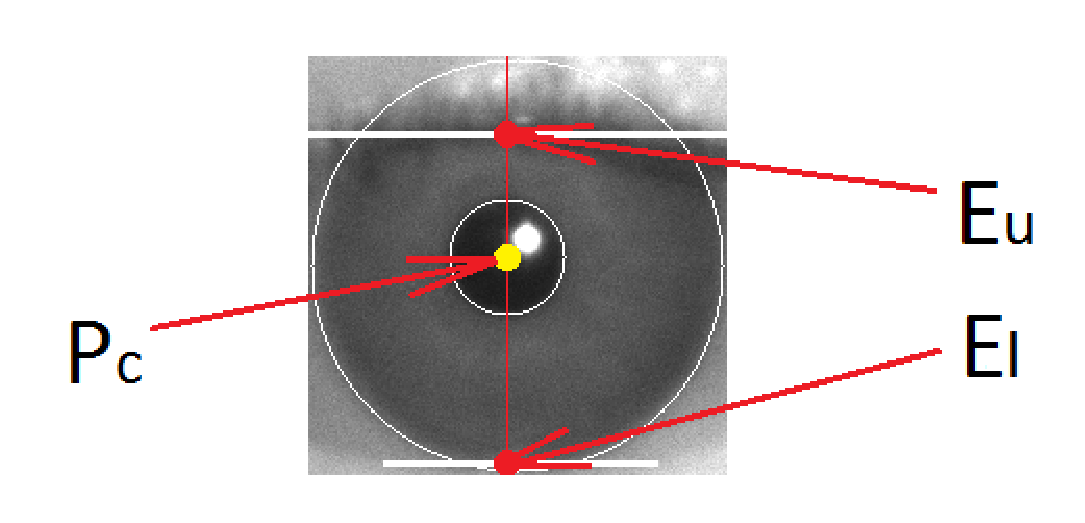
\includegraphics[width=0.5\columnwidth]{pictures/eyelid_position_pointers.eps}
	\caption{Определение положения верхнего $E_u$ и нижнего $E_l$ век, $P_c$ - центр зрачка}
	\label{fig:eyelid_position}
\end{figure}

\noindent
Вычисление промежуточного показателя качества является завершающей операцией первого блока и может производится различными способами. В данной работе в качестве оценки предлагается вычисление взвешенной суммы по нескольким накопленным в процессе обработки параметрам качества, среди которых: средние яркости полного кадра $I_{avg}^f$ и области глаза $I_{avg}^e$ (Рис.~\ref{fig:eyelid_position}), значение контраста на границе зрачок-радужка $C_{pi}$, степень открытости глаза $NEO$ (\ref{eq:neo_p}), выраженная по значениям $E_l$ и $E_u$ (Рис.~\ref{fig:eyelid_position}). Коэффициенты регрессии между набором используемых метрик и значением математического ожидания соответствующего распределения степени схожести для пар сравнений свой со своим предложено использовать в качестве весов для вычисления финального показателя качества.

Поскольку входные данные представляют собой видеопоследовательность, а не единичный кадр, можно выбирать изображения наилучшего качества в течение заранее определенного периода времени по завершению любого этапа алгоритма. Выбор может быть выполнен с использованием показателей качества, которые были оценены до помещения изображения в буфер (Рис.~\ref{fig:algorithm_structure}). После того как буфер полностью заполнен, каждый последующий кадр вытесняет один из кадров худшего качества в течение предопределенного времени. Как только заданное время истекло, выбранные изображения переносятся на второй этап обработки. В качестве временной константы может быть выбрано время полной обработки изображения на втором этапе.

Второй этап состоит из более вычислительно сложных операций. Обрабатываются только изображения из буфера. Этап начинается с поиска центра $(x_i,y_i)$ и радиуса $r_i$ радужки на изображении глаза с использованием информации о параметрах зрачка. Используемый подход к поиску аналогичен тому, что использовался для поиска зрачка. Информация о расположении век используется здесь для выбора диапазона углов при обходе контура интегро-дифференциальным оператором. Информация о положении век используется для определения области поиска интегро-дифференциальным оператором. Для удаления ресниц и частично затенений используется подход, описанный в~\cite{aligholizadeh_2011}. Далее над изображениями радужки полученной маски осуществляется операция нормализации (\ref{eq:certesian-polar}). Последним этапом второго блока является извлечение уникальных особенностей радужки и построение вектора признаков.

Извлечение особенностей радужки производится для каждого кадра, прошедшего все проверки по качеству. Заранее определенное количество векторов признаков, полученное в процессе регистрации ($N_E$) сохраняется в базе данных. Все они используются в дальнейшем для сравнения. Так как, возможность накапливать векторы признаков предлагается использовать и при верификации, существует несколько вариантов их использования. Метод сравнения <<каждый с каждым>> подразумевает $N_E \times N_V$ количество сравнений, а это не всегда оправдано ($N_V$ - текущее количество векторов признаков в режиме верификации). Для того чтобы уменьшить количество сравнений, несколько векторов признаков могут быть отобраны в качестве наиболее репрезентативных. Правило отбора таких векторов основано на измерении для них степени схожести внутри одного класса. Пара векторов, для которых степень схожести минимальна выбираются в качестве образцов для последующего сравнения с векторами, хранящимися в базе данных. Таким образом количество сравнений уменьшается и становится равным $0.5*N_V(N_V-1)+2N_E$. Если для $N_E$ и $N_V$ выполняется условие $N_E > N_V/2$, то количество сравнений значительно уменьшается.


\subsection{Оценка качества изображения радужки}
\label{subsec:quality_assessment}

Оценка качества изображения является неотъемлемым этапом распознавания~\cite{matveev_doctor_thesis}. В литературе известно множество подходов к оценке качества изображения радужки~\cite{czajka_2013,chen_2012,galbally_2012,feddaoui_2011}. Однако, большинство из них не рассматривает мобильные приложения.
Подход, описанный в данной работе, имеет несколько ключевых особенностей по сравнению с методами, известными ранее~\cite{hamza_patent_2012,prabhakar_patent_2013}.

Главной особенностью решения является предложенный набор критериев качества изображения радужки. Набор составлен из метрик, позволяющих оценивать качество с учетом большинства возможных сценариев использования устройства. Оценка по каждому из критериев производится сразу после того, как произведено соответствующее измерение.

Персональное мобильное устройство подразумевает постоянное взаимодействие с пользователем. По этой причине второй особенностью предложенного решения является способность осуществлять обратную связь с пользователем устройства. В случае отсеивания кадра по какому-либо критерию качества, пользователю автоматически выводится подсказка в понятной для него форме. Например, если вычисленное расстояние до лица выходит за заранее определенный допустимый предел, то пользователю будет предложено расположить устройство ближе либо дальше.

\begin{figure}[t!]
	\centering
	\includegraphics[width=0.95\columnwidth]{pictures/qa_structure.png}
	\caption{Общая схема алгоритма оценки качества изображения}
	\label{fig:qa_structure}
\end{figure}

Оценка качества также позволяет поддерживать обратную связь не только с пользователем, но и с аппаратной частью устройства, обеспечивая корректировку параметров системы регистрации изображения, с целью получения кадров наилучшего качества (подробнее в заявке на изобретение~\cite{gnatyuk_patent_2018}). Например, изображение области глаза было классифицировано как переэкспонированное. Алгоритм автоматически корректирует значение экспозиции для регистрации последующего кадра. На схеме (Рис.~\ref{fig:qa_structure}) изображена структура алгоритма оценки качества изображения. Обратная связь с пользователем и аппаратной частью условно обозначена буквой $F (feedback)$ со стрелкой.

\subsection{Использование дополнительных сенсоров}
\label{subsec:sensor_usage}

Отличительной особенностью метода является использование информации с дополнительных сенсоров, доступных для использования внутри устройства. Так, например, информация об уровне освещенности, данные с дальномера и иные доступные данные могут быть использованы для подстройки как параметров аппаратной части устройства, так и алгоритма. Таким образом реализуется связь между ключевыми компонентами биометрической системы: пользователем, аппаратной и программной частями устройства (Рис.~\ref{fig:hw_sw_user_scheme}). Детальное описание предложенного метода приведено в заявке~\cite{odinokikh_patent_2017_irec_ru}.

\begin{figure}[t!]
	\centering
	\includegraphics[width=0.95\columnwidth]{pictures/hw-sw-user-scheme.png}
	\caption{Условная схема взаимодействия между элементами системы распознавания}
	\label{fig:hw_sw_user_scheme}
\end{figure}

Вводятся дополнительные метрики оценки качества, позволяющие ускорить процесс обработки информации внутри алгоритма. Обе преложенные метрики (\ref{eq:neo_p}, \ref{eq:neo_i}) описывают уровень открытости глаза на различных этапах алгоритма с использованием информации о положении век $E_u$ и $E_l$.

\begin{equation}\label{eq:neo_p}
	NEO_p=\frac{|E_l-E_u|}{R_p}
\end{equation}

\begin{equation}\label{eq:neo_i}
	NEO_i=\frac{|E_l-E_u|}{R_i}
\end{equation}

\noindent
Метрики $NEO_p$ и $NEO_i$  (NEO, сокр. - normalized eye opening) вычисляются и используются на разных этапах алгоритма, сразу, как только информация о значения радиусов зрачка $R_p$ и радужки $R_i$ становится доступной. Введение пары метрик позволяет оценивать уровень открытости глаза на ранних этапах алгоритма и показало свою полезность на практике.

Заключительным этапом алгоритма является построение вектора признаков с применением фильтра Габора к нормализованному изображению радужки, а также метода адаптивного квантования, подробно описанного в главе~\ref{sec:gabor-and-quantization}. Параметры фильтра подобраны в результате оптимизации методом Нелдера-Мида на обучающей выборке.

{\bf Экспериментальные результаты}

Экспериментальные результаты включают в себя оценку точности и скорости распознавания, а также описание данных, использованных для оценки.

{\bf Описание базы данных}

На сегодняшний день не существует достаточно представительных баз данных изображений радужных оболочек глаза, полученных в БИК области частот, достаточных для того, чтобы произвести комплексную оценку метода с учетом изменений условий окружения, учитывающих особенности поведения пользователя, цвет глаз и т.д. По этой причине для проведения исследований и разработки была собрана собственная база данных. Каждый биометрический образец представлен пятисекундным видеороликом, отражающим попытку регистрации/верификации. Детальная информация о собранной БД представлена в Таб.~\ref{tab:dataset_spec}.

\begin{table}[h]
	\begin{center}
		\small
		\begin{tabular}{l|c|c}
			\hline
			Параметры										& Без очков		  & С очками \\
			\hline
			Количество пользователей						& 286             & 123 \\
			Количество радужек								& 566             & 222 \\
			Число сравнений									& 27\,149\,310    & 2\,936\,082 \\
			Расовая принадлежность							&  \multicolumn{2}{c}{Азиаты \& Европеоиды} \\
			Количество глаз в кадре							&  \multicolumn{2}{c}{один глаз} \\
			Количество видеороликов на каждый глаз			&  \multicolumn{2}{c}{$\leq$10} \\
			Количество кадров в видеоролике					&  \multicolumn{2}{c}{75} \\
			Расстояние съемки								&  \multicolumn{2}{c}{$15 - 35$ (см)} \\
			Разрешение матрицы камеры       				&  \multicolumn{2}{c}{$1280 \times 720$} \\
			\hline
		\end{tabular}
	\end{center}
	\caption{Характеристики использованной базы данных}
	\label{tab:dataset_spec}
\end{table}


База данных собрана с использованием мобильного устройства (планшета), оснащённого встроенной компактной камерой, работающей в БИК диапазоне, и активной БИК-подсветкой. Для сбора был установлен следующий сценарий: пользователь берёт устройство на начальном расстоянии около 35 см; начинается запись видеоролика и пользователь приближает устройство ближе к глазу до расстояния 15 см в течение 5 секунд. Такой подход был выбран из соображений возможных особенностей взаимодействия пользователя с устройством, таких как более удобное расстояние, возможное дрожания рук и т.д.

\begin{figure}[!h]
	\centering
	\begin{subfigure}{.475\textwidth}
		\centering
		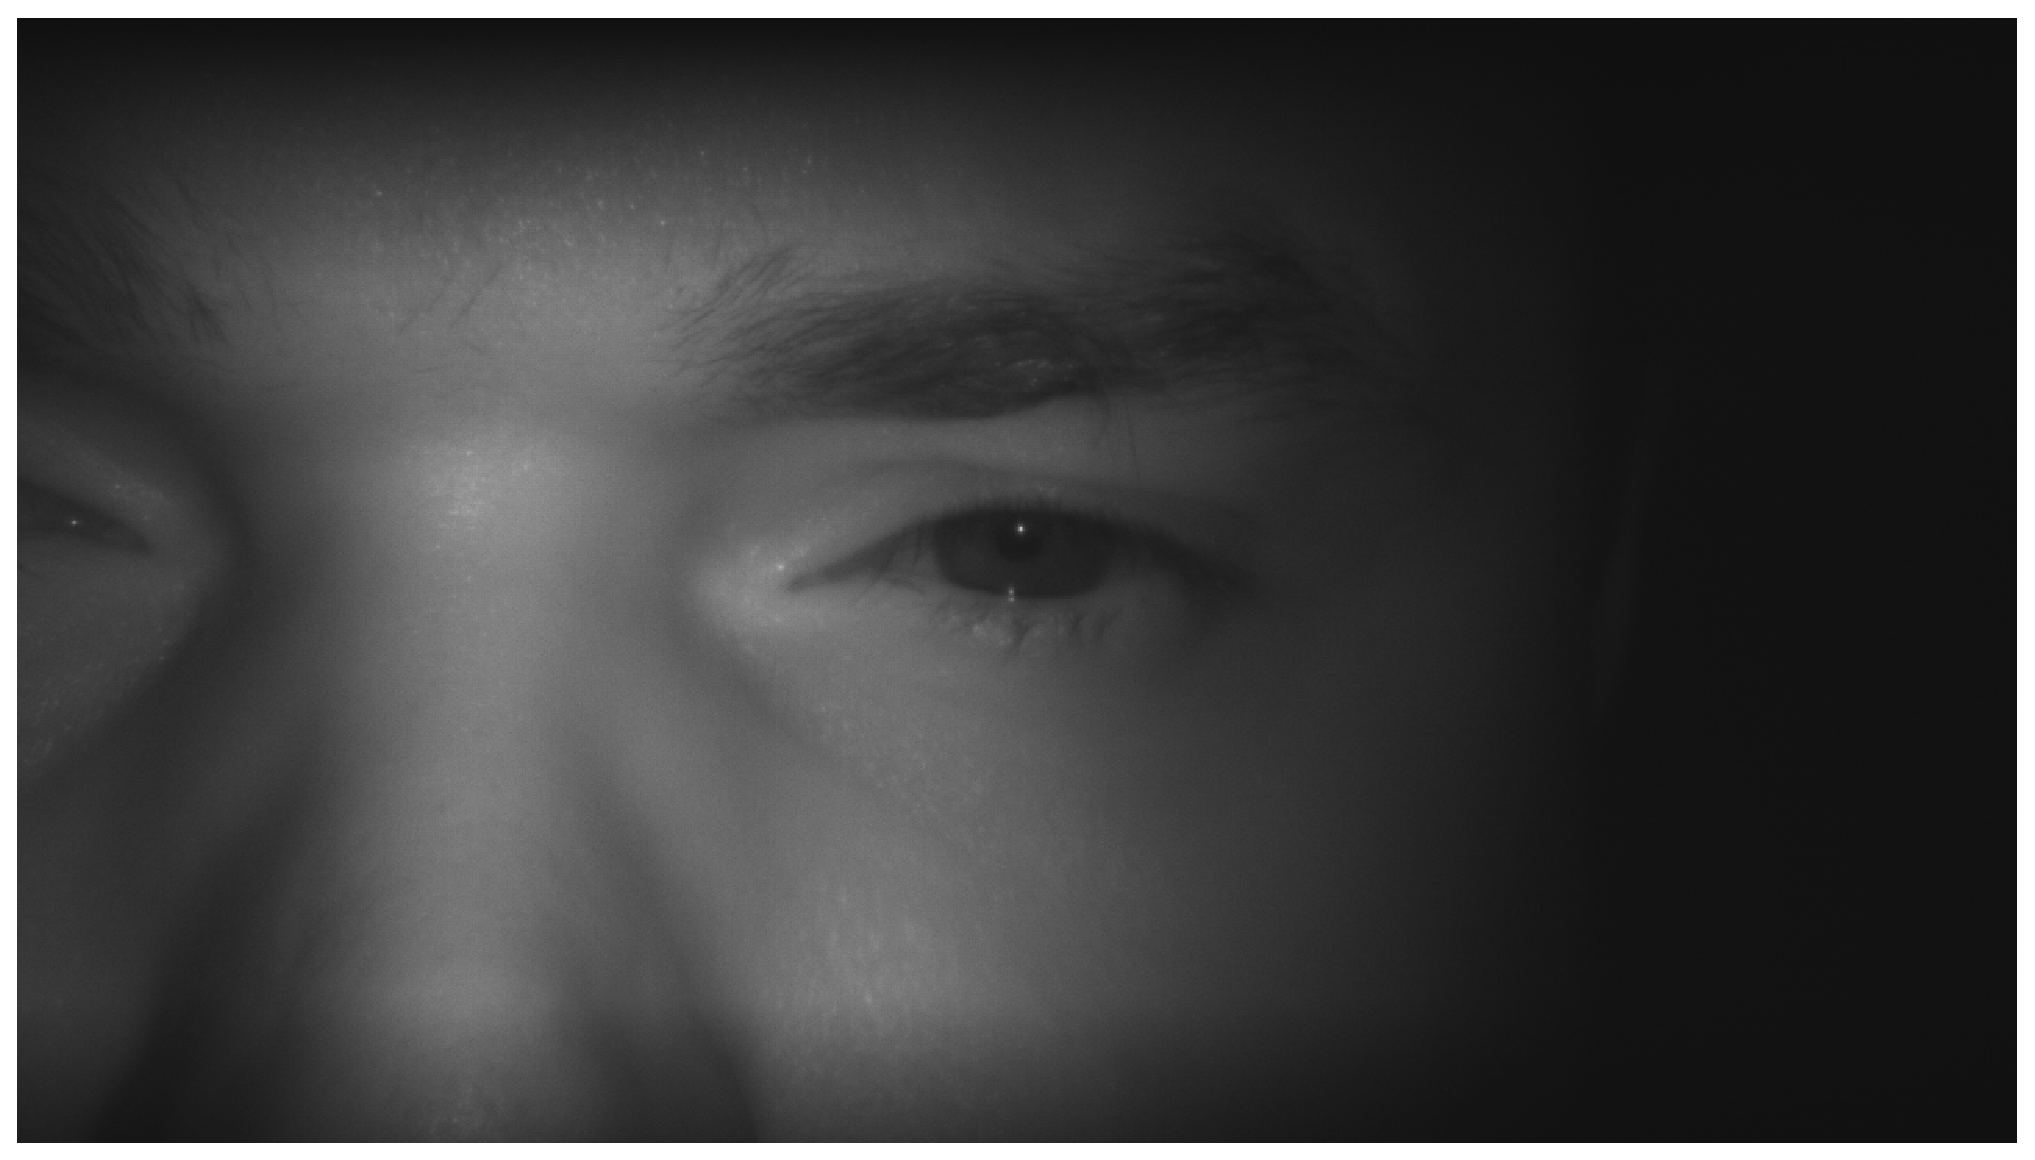
\includegraphics[width=0.95\columnwidth]{pictures/mobile_db_example_30.eps}
		\label{fig:mobile_db_example_18}
	\end{subfigure}%
	\begin{subfigure}{.475\textwidth}
		\centering
		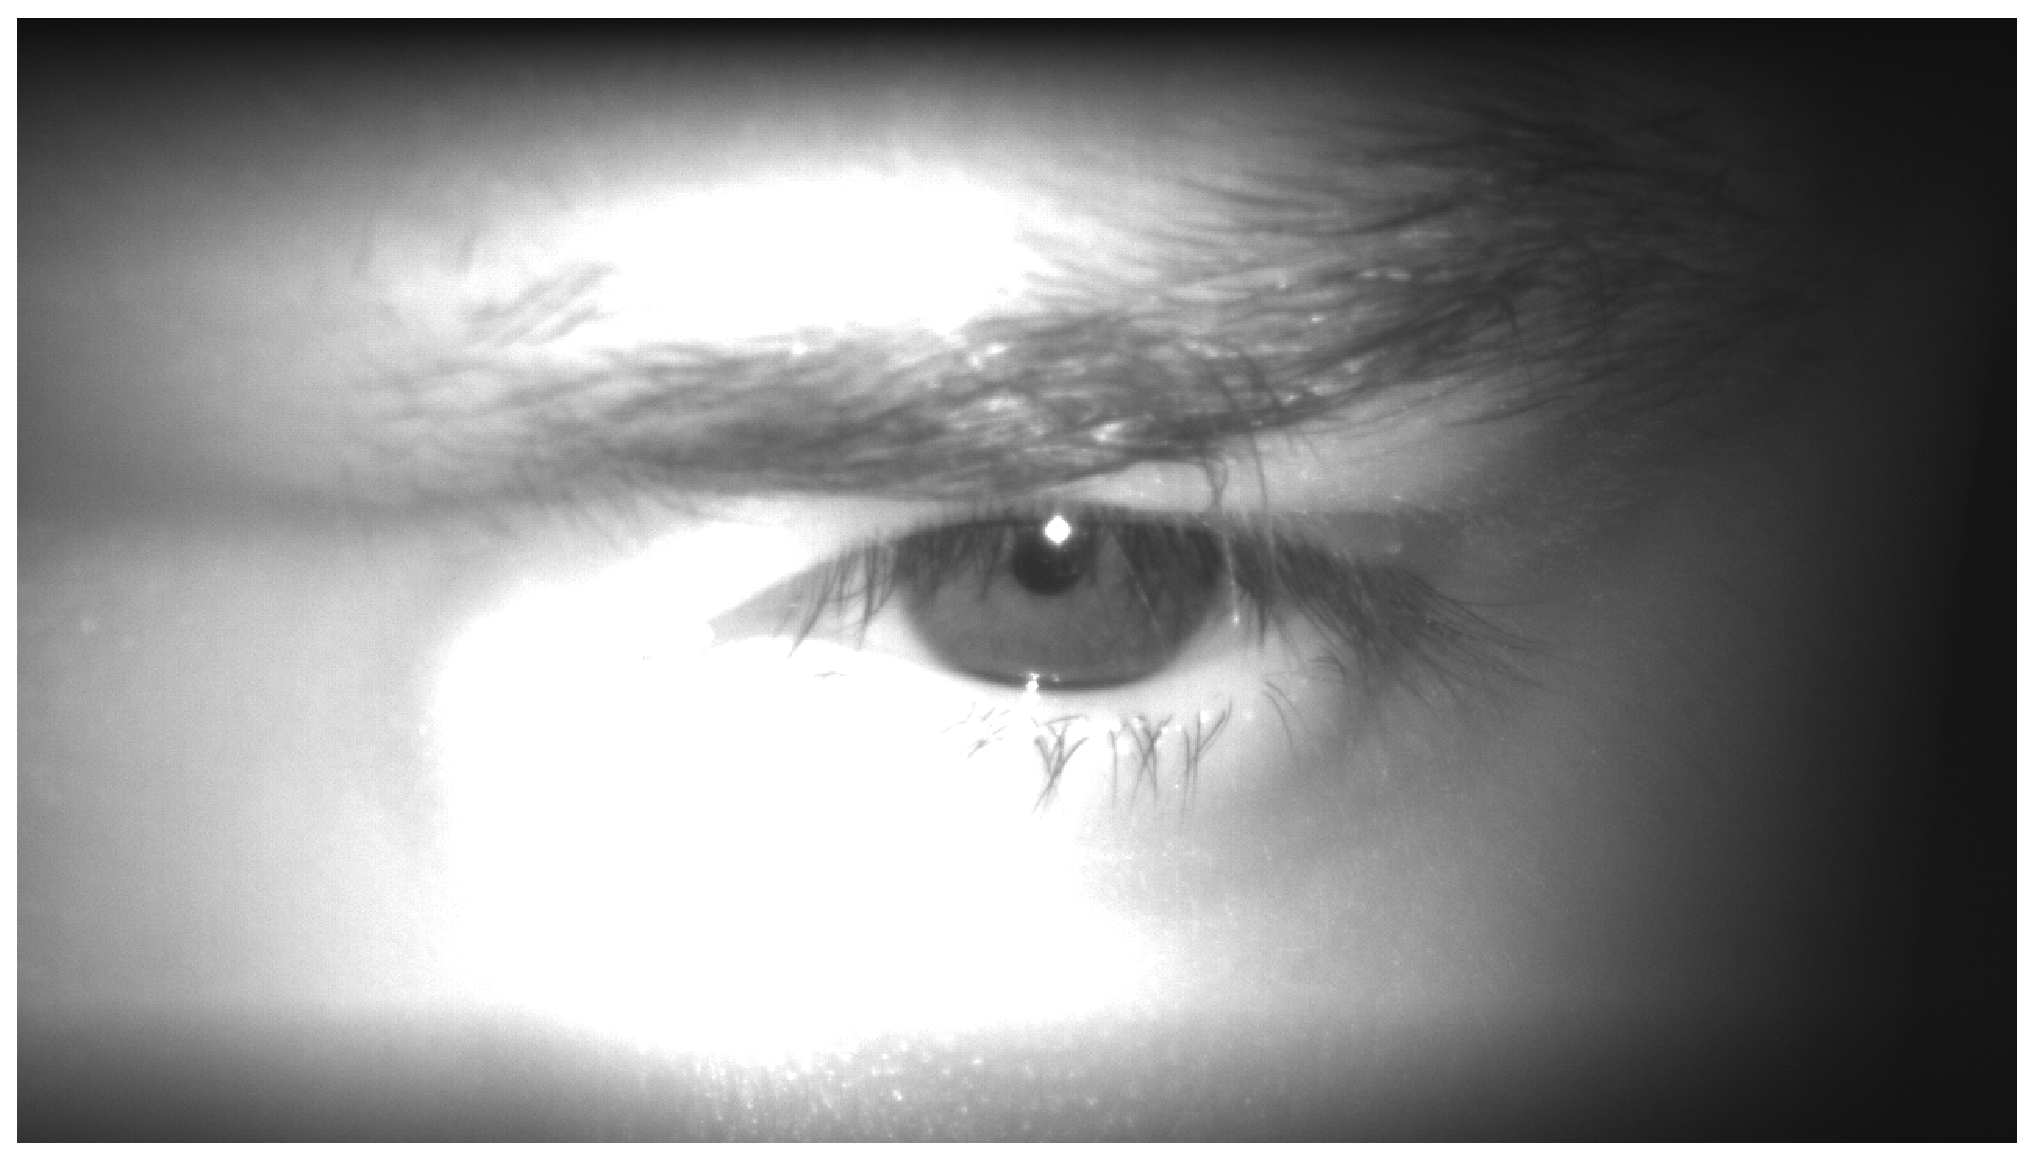
\includegraphics[width=0.95\columnwidth]{pictures/mobile_db_example_18.eps}
		\label{fig:mobile_db_example_30}
	\end{subfigure}%
	\caption{Примеры изображений, полученных на разных расстояниях от лица до устройства: 18 и 30 (см) слева и справа соответственно}
	\label{fig:mobiel_db_examples}
\end{figure}

Примеры изображений, снятых камерой, представлены на Рис.~\ref{fig:mobiel_db_examples}. Изображения взяты из одной и той же видеопоследовательности, но соответствуют разным расстояниям (18 и 30 см). Все видеопоследовательности используются для моделирования попыток регистрации и верификации. Для обоих сценариев использовались одни и те же параметры алгоритма, поэтому значение $FTE$ равно значению $FTA$ (Таб.~\ref{tab:accuracy_results}).

{\bf Результаты по точности распознавания}

В соответствии с общепринятыми понятиями и определениями, подробно описанными, например, в~\cite{dunstone_biosystem}, а также стандартах ISO/IЕС 19795-1:2006, ISO/IEC 19794-6:2011 и ГОСТ Р ИСО/МЭК 19795-1-2007, для оценивания производительности системы распознавания были выбраны следующие (основные):

\begin{itemize}
	\setlength\itemsep{0.01em}
	\item[$\bullet$] FTE (failure to enroll) - количество транзакций регистрации, для которых не возможно завершить извлечение биометрического эталона;
	\item[$\bullet$] FTA (failure to acquire) - количество транзакций верификации, для которых не возможно завершить извлечение биометрического эталона;
	\item[$\bullet$] Степень схожести - численная мера близости двух биометрических эталонов;
	\item[$\bullet$] FNMR (false non-match rate) - вероятность ложного несовпадения;
	\item[$\bullet$] FMR (false match rate) - вероятность ложного совпадения;
	\item[$\bullet$] EER (equal error rate) - равный уровень ошибок, коэффициент, при котором FNMR=FMR;
	\item[$\bullet$] Enrollment template - биометрический шаблон, полученный в режиме регистрации, содержащий один или несколько биометрических эталонов;
	\item[$\bullet$] Probe template - биометрический шаблон, полученный в режиме верификации, содержащий один или несколько биометрических эталонов;
\end{itemize}

Полученные результаты по точности распознавания предложенного алгоритма представлены в таблице~\ref{tab:accuracy_results}. Данные значения были получены с использованием системы автоматического тестирования и базы данных, описанной в таблице~\ref{tab:dataset_spec}.

{\bf Процедура тестирования} состояла из нескольких этапов:
\begin{enumerate}
	\setlength\itemsep{0.01em}
	\item Формирование биометрических эталонов из всех видеопоследовательностей в режиме регистрации;
	\item Формирование биометрических эталонов из всех видеопоследовательностей в режиме верификации;
	\item Формирование списка всех возможных пар сравнений шаблонов (enrollment-probe);
	\item Вычисление значений степени схожести для каждой из пар биометрических шаблонов;
	\item Вычисление показателей точности распознавания (Таб.~\ref{tab:accuracy_results});
\end{enumerate}

Оценка FTA и FTE производится по результатам выполнения шагов 1 и 2. Полученные значения (Таб.~\ref{tab:accuracy_results}) отражают возможность метода обрабатывать данные, полученные в сложных условиях.

Поскольку система аутентификации представляет собой бинарный классификатор, точность распознавания для нее оценивается с помощью ROC (receiver operating characteristic) кривой, отражающей зависимость между величинами FMR и FNMR~\cite{enc_biometrics}. Значения FMR и FNMR изменяются в зависимости от внутренних параметров системы распознавания, таких как порог принятия решения, с которым сравнивается полученное значение степени схожести биометрических эталонов, а также самих значений степени схожести. Более подробно о процедуре оценивания описано в работе~\cite{odinokikh_hprec_2018}.


\begin{table}[h]
	\begin{center}
		\small
		\begin{tabular}{|l|c|c|}
			\hline
			Значение	& Без очков   	& С очками\\
			\hline
			FTA/FTE		& 0.0685        & 0.07001 \\
			FMR			& $10^{-7}$     & $10^{-6}$ \\
			FNMR		& 0.01077       & 0.03912 \\
			EER			& 0.00128       & 0.00574 \\
			\hline
		\end{tabular}
	\end{center}
	\caption{Результаты по точности распознавания}
	\label{tab:accuracy_results}
\end{table}

{\bf Результаты по скорости распознавания}

Производительность метода оценивалась при помощи вышеупомянутого планшета, оснащенного процессором Qualcomm Snapdragon 800 (2.26 GHz, Quad-core). Измерения производились на одном ядре процессора. Медианное время выполнения составило 25 и 42 (мсек) для операций первого и второго блоков (\ref{subsec:algorithm_structure}, Рис.~\ref{fig:algorithm_structure}) соответственно.

\section{Выводы ко второй главе}

Рассмотрены основные трудности, связанные с биометрическим распознаванием человека по радужной оболочке глаза при помощи мобильного устройства. Предложены, протестированы и внедрены:

\begin{enumerate}
	\item новая многостадийная структура алгоритма для автоматического распознавания, построенная с использованием промежуточных блоков оценки качества изображения, позволяющая осуществлять распознавание человека при помощи устройства со значительно ограниченной вычислительной мощностью в режиме реального времени ($\approx15$ кадров/сек.), удовлетворяющая критериями ошибок: $FNMR\leq1\%$ при $FMR<10^{-7}$;
	\item алгоритм оценки качества, позволяющий:
	\begin{itemize}
		\item[$\bullet$] комплексно оценивать качество входящего изображения радужки на предмет его пригодности для извлечения признаков и формирования биометрического эталона;
		\item[$\bullet$] обеспечивать обратную связь с пользователем путем отображения подсказок, понятных пользователю, на экране устройства, на основании внутренних измеряемых показателей качества изображения;
		\item[$\bullet$] производить управление параметрами системы регистрации изображения с целью получения изображения радужки наилучшего качества;
		\item[$\bullet$] учитывать и использовать данные с иных доступных сенсоров, позволяющих получать дополнительную информацию об окружении.
	\end{itemize}
\end{enumerate}

%% Глава 3
\chapter{Выделение области радужки на изображении}
\label{chapter:segmentation}

Выделение (сегментация) области радужки на изображении -- один из основных этапов распознавания. Ошибки сегментации влекут за собой рост числа ошибок распознавания, делая систему менее надежной и удобной в использовании. Подавляющее большинство существующих подходов ориентированы на использование систем в условиях слабо изменяющегося окружения. Классические методы, основанные на эвристиках, хорошо зарекомендовали себя здесь. Широкое распространение технологий распознавания создает необходимость обеспечения полной функциональности систем в более широком диапазоне условий и, как следствие, создания более гибких и устойчивых решений.

\section{Особенности выделения радужки в сложных условиях}
\label{sec:hard_condition_segm_features}

Сложные условия окружения, характерные для сценария взаимодействия пользователя с мобильным устройством, оказывают значительное влияние не только на свойства самого биометрического признака, но и на качественные характеристики изображения, из которого следует предварительно извлечь информацию, описывающую его уникальные особенности.

Факторы окружения в особенной степени существенны для биометрической системы, использующей изображение объекта распознавания в качестве входных данных, в особенной при распознавании по радужке: уровень окружающего освещения варьируется в диапазоне от $10^{-4}$ в ночное время суток или темном помещении до $10^5$ (лк) в полдень под прямыми солнечными лучами; распределение освещенности в области радужки, определяемое характеристиками и расположением источников света относительно лица и радужки. Изменение размеров зрачка приводят к деформации структуры радужки, различные погодные условия вынуждают пользователя устройства моргать, сильно прищуривать глаза и могут значительно снизить качество изображения в целом. Факторы окружения, влияющие на распознавание, подробно описаны в литературе~\cite{raja_2014,thavalengal_2016,btas_competition_2016,odinokikh_2018}, а некоторые примеры изображений радужки, получаемых в сложных условиях, приведены на Рис.~\ref{fig:iris-mobile-img-examples} и~\ref{fig:iris_iamge_quality_degradation}.

\begin{figure}[t!]
	\centering
	\includegraphics[width=0.95\columnwidth]{pictures/iris-mobile-img-examples.png}
	\caption{Примеры изображений полученных при помощи мобильного устройства: причина (снизу) и следствие (сверху)}
	\label{fig:iris-mobile-img-examples}
\end{figure}

Важной особенностью распознавания при помощи мобильного устройства являются поведенческие характеристики пользователя, описанные в главах~\ref{sec:mobile_iris_features} и~\ref{sec:main_difficulties_mobile}. Примеры ошибок выделения области радужки на изображении в следствие влияния факторов окружения и особенностей поведения пользователя приведены на Рис.~\ref{fig:iris_iamge_quality_degradation}.

\section{Методы выделения радужки на изображении}
\label{sec:segm_method}

\subsection{Обзор существующих методов}
\label{sec:segm_existing_app_overview}

Существует большое количество различных методов и подходов к решению задачи выделения области радужной оболочки глаза на изображении. Методы хорошо зарекомендовали себя для не мобильных приложений. Многие из них используются в коммерческих решениях и распространены настолько широко, что их по праву можно называть классическими.

Среди классических методов можно выделить основные направления:
\begin{enumerate}
	\item[$\bullet$] Применение интегро-дифференциального оператора (\ref{eq:daugman_ido}), предложенного в работе~\cite{daugman_how_works}. Оператор используется для выделения радиально-симметричных структур, которыми, в данном случае, предлагается описывать зрачок и радужку. Метод имеет высокие точность и устойчивость, но обладает неприемлемой для большинства приложений вычислительной сложностью~\cite{matveev_doctor_thesis}. Примеры использования~\cite{bakhtiari_2006,adam_2008,barzegar_2008}. Примеры совершенствования исходного решения путем добавления различных методов предобработки представлены в работах~\cite{alonso_11,alonso_12,hu_11,jeong_10,mahadeo_12};
	\item[$\bullet$] Анализ гистограммы изображения, бинаризации и последующее оценивание радиусов зрачка и радужки~\cite{guang_2007,pan_2007,ling_2010}. Методы показали свою работоспособность на качественных изображениях~\cite{casia_v3,bath_2005}, однако, в сложных условиях~\cite{ndiris_2010,ubiris_2005} их применение сильно ограничено;
	\item[$\bullet$] Методология Хафа (Hough), позволяющая оценить параметры кривых заданного вида (в данном случае окружностей, описывающих зрачок и радужку) с использованием т.н. аккумуляторов. В качестве примеров использования различных подходов внутри методологии можно привести следующие~\cite{wildes_1997,proenca_2006,basit_2007,boyd_2010}. Данный подход позволяет получить выигрыш по скорости обработки, но гораздо менее устойчив к зашумлённым данным в сравнении, например, с методами, использующими интегро-дифференциальный оператор.
\end{enumerate}

Существенная часть работ, посвящённых выделению области радужки за последнее время и приходящаяся на период с 1997 по 2014 годы, сосредоточена вокруг вышеперечисленных методов~\cite{korobkin_odinokikh_segm_2018}. В работах предлагаются различные варианты улучшения методологий путем добавления процедуры специальной предобработки изображения~\cite{yuan_2005,pan_2007}, решающих правил, основанных на всевозможных эвристиках~\cite{matveev_doctor_thesis,daugman_how_works,ma_2004,zhou_2004,bowyer_survey_2008,moravcik_2010}, а также техник машинного обучения. Общая схема классического подхода изображена на Рис.~\ref{fig:segm-classic-approach} Методы хорошо разобраны и классифицированы по различным особенностям в работе~\cite{matveev_doctor_thesis}.

\begin{figure}[h!]
	\centering
	\includegraphics[width=0.95\columnwidth]{pictures/segm-classic-approach.png}
	\caption{Общая схема классического подхода к выделению радужки на изображении)}
	\label{fig:segm-classic-approach}
\end{figure}

С увеличением количества всевозможных данных для обучения и развитием аппаратных средств область машинного обучения в недавнем времени претерпела существенные изменения. Глубокое обучение (deep learning, DL) стало одним из подходов, позволяющих эффективно использовать данные большие объемы данных. Начиная с 2012 года глубокое обучение и, в частности, глубокие сверточные нейронные сети (deep convolutional neural networks, deep CNN) были успешно применены для решения целого ряда задач компьютерного зрения, достигнув результатов, в значительной степени превосходящих полученный ранее существующими методами и даже человека~\cite{krizhevsky_2012,girshick_2014,toshev_2014,karpathy_2014}.

Прошло некоторое время, пока глубокое обучение достигло области биометрического распознавания и было применено для выделения радужки на изображении. На сегодняшний день создание различных приложений, в том числе мобильных, требует от алгоритма высокой устойчивости к сильно изменяющимся условиям окружения, упомянутым ранее (\ref{sec:main_difficulties_mobile}). Авторы~\cite{liu_2016} впервые продемонстрировали преимущества подхода к сегментации радужки с использованием свёрточных нейронных сетей, в частности, на изображениях радужек, полученных в более сложных условиях. В работе также сравниваются два основных подхода к сегментации с использованием сверточных сетей: так называемый <<patch-based>> подход, при котором сеть обучают с использованием небольших фрагментов исходного изображения, принадлежащих либо не принадлежащих области объекта, который необходимо выделить, присваивая каждому из фрагментов марку класса в зависимости от принадлежности; вторым подходом является т.н. <<end-to-end>> способ обучения, когда на вход сети подается полноразмерное изображение, а выходом её является бинарная маска той же размерности, значение каждого пикселя в которой определяет класс объекта, например: 1 - радужка, 0 - фон.

Иным примером <<patch-based>> подхода является архитектура, представленная в работе~\cite{arsalan_2017}. Незадолго до её появления, исследователи в~\cite{shelhamer_2017} показали, что такой подход и предложенный метод обучения в значительной степени ухудшают качество сегментации, в очередной раз закрепив преимущества <<end-to-end>> подхода. В работе~\cite{jalilian_2017} продемонстрирована возможность использования архитектуры SegNet применительно к сегментации радужки, а также предложено использование техники дропаут (dropout) обучения, впервые описанной в работе~\cite{wang_2013}. Подход позволил достигнуть достаточно высокой точности сегментации, однако, в виду вычислительной сложности, не применим на практике. Иная CNN архитектура была представлена в работе~\cite{bazrafkan_2018}. Предложено исключение пулинг (pooling) слоёв, показана высокая эффективность. Однако, в работе~\cite{krizhevsky_2012} ранее утверждалось, что такой подход не позволяет извлекать сложные особенности из изображения, что критично для задачи сегментации в сложных условиях. Известно также, что отсутствие пулинг слоёв приводит к тому, что построенная на таком подходе архитектура оказывается чувствительной к различным сдвигам объекта на изображении.

\subsection{Выделение области радужки методами глубокого обучения}
\label{sec:segm_proposed_method}

В настоящей работе предложены новые CNN архитектуры. За основу взяты две базовые архитектуры, демонстрирующие лучшие результаты в задаче сегментации различных объектов на изображении: FCN (fully-convolutional network) и SegNet. Предложена новая структура основных блоков, из которых состоят обе архитектуры.

{\bf Основные подходы с использованием глубокого обучения}
\label{sec:segm_basic}

Архитктура FCN, впервые предложенная для решения задач семантической сегментации объектов, подразумевает полное исключение полносвязных (fully-connected) слоев~\cite{shelhamer_2017}. Это свойство позволяет адаптировать модель, обученную для решения задачи классификации, в модель, решающую задачу сегментации объектов без дополнительных оптимизаций. Архитектура поддерживает оба (patch-based и end-to-end) подхода к обучению и представляет собой модель т.н. <<кодировщик-декодировщик>> (encoder-decoder), изображенную на Рис.~\ref{fig:encoder-decoder-architecture}. Роль кодировщика заключается в построении высокоуровневого представления входных данных, в то время как декодировщик осуществляют обратную задачу. Принимая на вход представление, полученное кодировщиком, декодировщик переводит его в пространство размерности исходного изображения, используя закодированную информацию о пространственном соотношении различных элементов текстуры изображения.
В архитектуре FCN декодировщик построен с использованием блоков, содержащих слои деконволюции или (deconvolution layers) или транспонированные свёрточные слои, предложенные в работе~\cite{zeiler_2011}.
Выход каждого деконвоюционного слоя объединяется с картами признаков соответствующих симметричных слоёв кодировщика с использованием т.н. пропускных соединений (skip-connections) (Рис.~\ref{fig:encoder-decoder-architecture}) с целью восстановления структурной информации.

\begin{figure}[t!]
	\centering
	\includegraphics[width=0.95\columnwidth]{pictures/dec_enc.png}
	\caption{Общая схема архитектуры кодировщик-декодировщик (encoder-decoder)}
	\label{fig:encoder-decoder-architecture}
\end{figure}

Другим примером архитектуры, реализующей схему кодировщик-декодировщик выступает SegNet~\cite{badrinarayanan_2017}. Основным вкладом работы стала замена вычислительно-сложных и требовательных к памяти устройства операций деконволюции так называемыми <<unpooling>> слоями. Большая требовательность по объему потребляемой памяти для FCN обусловлена тем необходимостью хранить карты признаков, являющихся выходами каждого из блоков кодировщика до тех пор, пока они не будут использованы декодировщиком. Таким образом, пик потребления памяти устройства архитектурой достигается в момент, когда все карты признаков кодировщика извлечены, т.е. в момент формирования вышеупомянутого высокоуровневого представления. Архитектура SegNet позволяет на порядки снизить количество памяти, необходимой для полного прямого прохода. Несмотря на преимущества, подход SegNet с unpooling слоями снижает емкость сети, а невозможность пропускать градиенты через skip-connection при обратном распространении ошибки затрудняют обучение. Разница между структурами блоков декодировщика FCN и SegNet проиллюстрирована на Рис.~\ref{fig:fcn-segnet}.

\begin{figure}[t!]
	\centering
	\includegraphics[width=0.95\columnwidth]{pictures/fcn_segnet.png}
	\caption{Структуры основных блоков декодировщиков FCN (справа) и SegNet (слева)}
	\label{fig:fcn-segnet}
\end{figure}

{\bf Структура основных блоков архитектуры}
\label{sec:segm_proposed_blocks}

Изначально идея использования остаточных (residual) связей при конструировании блоков была предложена в контексте очень глубоких сетей~\cite{he_2016}. Далее, остаточные блоки хорошо зарекомендовали себя как эффективно использующие память и позволяющие при этом поддерживать достаточную ёмкость. Их обходные (bypass) соединения способствуют эффективной передаче градиента при обратном распространении и позволяют оптимизировать также добавочную часть в каждом соединении. Общая структура остаточного блока приведена на Рис.~\ref{fig:gen-resnet}. Авторы~\cite{he_2016} также предложили сразу несколько модификации блока, отличающихся количеством каналов и глубиной (Рис.~\ref{fig:res-types}).

\begin{figure}[h!]
	\centering
	\includegraphics[width=0.45\columnwidth]{pictures/general_resnet.png}
	\caption{Общая структура остаточного (residual) блока}
	\label{fig:gen-resnet}
\end{figure}

Предложено дополнение блоков слоями нормализации (batch normalization), впервые описанными в работе~\cite{ioffe_2015}, позволяющими ускорить сходимость модели и повысить её обобщающую способность, тем самым снижать чувствительность модели к вариациям входных данных.

\begin{figure}[t!]
	\centering
	\includegraphics[width=0.5\columnwidth]{pictures/res_types.png}
	\caption{Модификации остаточных (residual) блоков: simple - слева, bottleneck - справа}
	\label{fig:res-types}
\end{figure}

{\bf Предложенные архитектуры}
\label{sec:segm_proposed_architecture}

Обе вышеупомянутые архитектуры (FCN, SegNet) были взяты за основу и модифицированы. SegNet по заявлению авторов~\cite{badrinarayanan_2017} позволяет обеспечить относительно низкое потребление памяти, хотя это во многом зависит от целевой платформы и вычислительных средств. С другой стороны FCN демонстрирует лучшую показатели сходимости. Архитектура ResNet-26 с блоками типа simple была взята в качестве кодировщика и симметрично-отражённая (Рис.~\ref{fig:encoder-decoder-architecture}) как декодировщик для модифицированной FCN. Предложенная модификация SegNet представляет собой ResNet-18 кодировщик и симметрично-отражённый декодировщик (Рис.~\ref{fig:encoder-decoder-architecture}). Блоки типа bottleneck были исключены из рассмотрения для применения в FCN, т.к. требовательны к размеру карт признаков на каждом последнем слое, что является существенной проблемой для FCN. Для FCN все слои max-pooling были заменены большими значениями смещений ядра в сверточных слоях (strided convolutions). В случае с SegNet max-pooling слои были перемещены в конец каждого блока кодировщика, а смещения ядер были выбраны единичными.

{\bf Экспериментальные результаты}
\label{sec:segm_exp_results}

Экспериментальные результаты были получены на двух наборах данных: публично доступном CASIA-Iris-Lamp-V3~\cite{casia_v3_lamp} и его модификации. Для оценки качества сегментации был выбран коэффициент Жаккара (Jacсard Index, IoU - intersection over Union,~\ref{eq:jaccard_index})~\cite{shelhamer_2017}. В качестве метода для сравнения был выбран метод, демонстрирующий наилучшие результаты~\cite{liu_2016}.

\begin{equation}
\label{eq:jaccard_index}
J(I_{pr},I_{gt}) = \frac{|I_{pr} \cap I_{gt}|}{|I_{pr} \cup I_{gt}| } = \frac{|I_{pr} \cap I_{gt}|}{|I_{pr}|+|I_{gt}|-|I_{pr} \cap I_{gt}|},
\end{equation}

\noindent
где $I_{pr}$ и $I_{gt}$  - множества пикселей, принадлежащих области радужки, предсказанных моделью и размеченными экспертом соответственно.

База данных изображений радужек CASIA-Iris-Lamp-V3 была выбрана в качестве основной для тестирования. Особенность этой БД в том, что в ней представлены изображения, полученные в осложненных, изменяющихся условиях окружения, позволяющие симулировать внутриклассовые отклонения: различные размеры зрачков, отвод взгляда, перепады яркости и др. База данных содержит 16212 изображений радужек 411 субъектов. Для оценивания методов были случайным образом выбраны 4865 изображений 124 субъектов. Разметка произведена экспертом с выполнением следующих условий: все пиксели, принадлежащие области радужки на изображении, а также ресницы, пересекающие область радужки, были приняты относящимися к классу <<область радужки>> (Рис.~\ref{fig:seg-results}). Область ресниц, перекрывающих радужку на изображении была также отнесена к классу радужки т.к. одной из основных целей работы было показать преимущества предложенных архитектур по сравнению с существующими. Сценарий был выбран именно таким, потому что позволил существенно упростить процедуру разметки и, таким образом, увеличить количество данных. База данных была предварительно поделена на три подвыборки: обучающую (train), валидационную (validation) и тестовую (test) в соотношении 3386, 478 и 1001 изображений соответственно. Результаты, полученные на валидационной выборке, использовались для выбора лучшей модели, которая затем оценивалась на тестовой.

\begin{figure}[t!]
	\centering
	\includegraphics[width=0.95\columnwidth]{pictures/seg-results.png}
	\caption{Результаты выделения области радужки}
	\label{fig:seg-results}
\end{figure}

Исследуемые модели обучались на протяжении 200 эпох пакетами (batch) изображений по 8 штук. В качестве алгоритма оптимизации был выбран Adam~\cite{kingma_2014}. Параметры обучения и тестирования были выбраны одинаковыми для всех исследуемых моделей.

Было проведено два эксперимента. В первом модели обучались на БД~\cite{casia_v3_lamp} без модификаций. Результаты представленные в Таб.~\ref{tab:seg-results}, демонстрируют что обе предложенные модели показывают примерно одинаково хорошие результаты, незначительно превосходя модель~\cite{liu_2016}.

\begin{equation}
\label{eq:random_contrast}
I'(x,y) = (I(x,y) - \overline{I}) \cdot C + \overline{I},
\end{equation}

\noindent
где $I(x,y)$ - исходное изображение, $\overline{I}$ - среднее значение яркости исходного изображения, $C$ - коэффициент изменения контраста.

Целью второго эксперимента была симуляция еще более значительных изменения окружения. С этой целью над исходным набором обучающих данных была произведена операция аугментации. Для этого над каждым изображением в обучающей выборке были выполнены следующие операции: значение контраста $C$ изменялось случайным образом в диапазоне $[50\%, 150\%]$ (~\ref{eq:random_contrast}), случайное значение в диапазоне $[-20\%, 20\%]$ также присваивалось интенсивности каждого пикселя. Финальное тестирование производилось на оригинальных изображениях из БД. Результаты показали, что предложенные модели значительное превосходят MFCN~\cite{liu_2016}, демонстрируя высокую устойчивость к изменениями условий окружения, а также высокую обобщающую способность. Несколько примеров результатов сегментации радужки на изображениях из CASIA-Iris-Lamp-V3 представлены на Рис.~\ref{fig:seg-results}.

\begin{table}[t]
	\begin{center}
		\begin{tabular}{|l|c|c|c|c|}
			\hline
			\multirow{2}{*}{Модель} & \multicolumn{2}{|c|}{Исх. набор данных, IoU} & \multicolumn{2}{|c|}{Модиф. набор данных, IoU} \\ \cline{2-5}
			\space 	& val. 	& test 	& val. 	& test set \\ \hline
			MFCN 	& $0.918$ 				& $0.919$ 				& $0.668$ 				& $0.676$ \\ \hline
			FCN 	& $0.930$ 				& $0.930$ 				& $0.884$ 				& $0.894$ \\ \hline
			SegNet 	& $0.928$ 				& $0.929$ 				& $0.916$ 				& $0.924$ \\ \hline
		\end{tabular}
		\caption{Результаты по точности выделения области радужки на изображении}
		\label{tab:seg-results}
	\end{center}
\end{table}

{\bf Результаты по скорости распознавания}
\label{sec:segm_results_speed}

Производительность метода оценивалась на процессоре Qualcomm Snapdragon 835 (2.45 GHz). Медианное время выполнения составило 35 мсек. Алгоритмическая сложность метода, при условии фиксирования её параметров (весов и смещений) и добавления операции масштабирования на входе, линейна по размеру входных данных.

\section{Выводы ко второй главе}

Рассмотрены особенности выделения области радужной оболочки глаза на изображениях, получаемых в сложных условиях окружения, связанных с использованием мобильного устройства и взаимодействия с пользователем. Приведен обзор и классификация существующих методов, обозначены их основные преимущества и недостатки. Рассмотрены новые методы, построенные с использованием методов глубокого обучения, выделены их основные преимущества, подчеркнуты перспективы использования и развития. Предложены, протестированы две новые архитектуры сверточных нейронных сетей, позволяющих производить устойчивое выделение области радужки на изображении низкого качества в сложных условиях окружения с частотой поступления кадров (15 кадров в секунду). Обе архитектуры позволили превзойти существующие, известные из литературы решения, основанные на глубоком обучении. Одна из предложенных архитектур успешно внедрена и используется в коммерческих продуктах.
%% Глава 4
\chapter{Методы извлечения и сравнения уникальных особенностей радужки}
\label{chapter:fem_methods}

Завершающими и неотъемлемыми частями алгоритма распознавания являются: извлечение уникальных особенностей (признаков) биометрического образца (-ов) и его (их) последующего сравнения, по результатам которого вычисляется степень схожести, используемая для принятия решения. Оба этапа обычно рассматриваются в едином контексте, т.к. являются смежными и сильно зависят друг от друга.

Извлекаемые признаки должны обладать следующими общими свойствами~\cite{jain_2004,matveev_doctor_thesis}:

\begin{enumerate}
	\item[$\bullet$] Уникальность (информативность/значимость): признаки должны содержать в себе информацию, достаточную для того, чтобы обеспечить отличаемость биометрического образца от других;
	\item[$\bullet$] Стабильность (устойчивость): неизменность во времени, независимость от условий регистрации и изменчивости самого образца;
	\item[$\bullet$] Применимость: признаки должны быть легко извлекаемыми, сравниваемыми и храниться в компактном виде.
\end{enumerate}

С точки зрения анатомии, для радужки можно выделить несколько основных источников для извлечения признаков: цвет радужки, форма зрачка, текстура радужки и др. Самыми информативным признаками радужки являются характеристики её текстуры~\cite{daugman_how_works}. Процедуре извлечения особенностей текстуры обычно предшествует этап нормализации (нормирования) изображения, представляющая собой конформное кольца радужки в прямоугольник, называемое полярным преобразованием (\ref{eq:certesian-polar}). Из литературы известно несколько вариантов такого преобразования, описанных в работе~\cite{arvacheh_2006}.

Обзоры различных методов извлечения и сравнения особенностей радужки приведены в работах~\cite{bowyer_survey_2008, bowyer_handbook_2012, ng_overview_2008, rathgeb_2011}. Среди модификаций можно выделить базовые подходы~\cite{matveev_doctor_thesis}: использование двумерных вейвлетов Габора~\cite{daugman_how_works}, использование матриц совместной встречаемости~\cite{gupta_2005,zaim_2006}, использование расположения и хаарктеристик ключевых точек текстуры~\cite{pranith_2010}, применение дискретного косинусного преобразования~\cite{monro_2007}, использование одномерный вейвлетов различных масштабов~\cite{boles_1998}, различные варианты преобразования Хаара~\cite{lim_2001,popescu_2011}, пирамиды Лапласа~\cite{wildes_1994}, метод основанный на ориентации градиентов~\cite{takano_2011}. В большинстве недавних работ предлагается использование методов глубокого обучения~\cite{liu_2016_di,gangwar_2016,proenca_2017,zhao_2017,tang_2017}.

Специфика использования мобильного устройства (\ref{sec:main_difficulties_mobile},~\ref{sec:mobile_iris_features}) сказывается на качестве выделения области радужки (\ref{sec:hard_condition_segm_features}) и изменчивости текстуры радужки (\ref{sec:iris-structure-and-properties},~\ref{sec:auth_method}). Следствием этих факторов является высокая вариативность входных данных для методов извлечения и сравнения этих особенностей. Это ограничивает возможности алгоритмов извлечения признаков, вызывая значительные внутриклассовые отклонения.

\section{Вейвлеты Габора и адаптивное квантование фазы}
\label{sec:gabor-and-quantization}

Одним из наиболее распространенных подходов извлечения особенностей и представления их в виде некоторого вектора признаков (т.н. эталона) радужки является использование вейвлетов Габора. В качестве входной информации используется нормализованное изображение радужки и бинарная маска, описывающая полезную и зашумленную (ресницы, веки, блики и др.) области изображения. Базовая структура такого подхода изображена на Рис.~\ref{fig:irec-basic-stages-gabor}.

\begin{figure}[ht!]
	\begin{center}
		\includegraphics[width=0.75\columnwidth]{pictures/irec-basic-stages-gabor.png}
		\caption{Общая схема алгоритма извлечения и сравнения признаков радужки при помощи вейвлетов Габора}
		\label{fig:irec-basic-stages-gabor}
	\end{center}
\end{figure}

Методы, основанные на применении вейвлетов Габора, являются одними из самых распространенных для не мобильных приложений, т.к. способны обеспечивать достаточную точность и надежность~\cite{daugman_how_works}. Процедура кодирования, присущая таким методам (Рис.~\ref{fig:fem-filter-and-quant}), необходима, в частности, для повышения стабильности представления вектора признаков и ускорения процесса сравнения. Одним из наиболее распространенных подходов к кодированию является бинарное квантование значений вектора признаков. Несмотря на то что квантование способно не учитывать нерелевантную, оно также способствует уменьшению полезной информации, дестабилизируя тем самым значения вектора признаков~\cite{hollingsworth_2009,proencca_2015}. Метод по-прежнему имеет одно важное преимущество, сделавшее его настолько популярным для использования: сравнение квантованных значений - битовая операция, а значит метод позволяет осуществлять сравнения с очень высокой скоростью. Эта особенность является очень важной, в частности, при решении задачи идентификации, когда требуется произвести поиск максимально похожего образца по базе данных, насчитывающей большое количество примеров.

\medspace
\begin{figure}[h]
	\begin{center}
		\includegraphics[width=0.95\columnwidth]{pictures/fem-filter-and-quant.png}
		\caption{Извлечение вектора признаков радужки вейвлетами Габора и последующее квантование}
		\label{fig:fem-filter-and-quant}
	\end{center}
\end{figure}

\noindent
Современные модификации подхода рассматривают понятие хрупкости как неустойчивость элементов вектора без учета характера появления такой неустойчивости. В работе предлагается разделение источников нестабильности на естественные и вызванные кодированием. Предлагается новый подход к построению вектора признаков радужной оболочки. Подход состоит из двух этапов: извлечения первичных признаков с использованием фильтрации единичным вейвлетом Габора, параметра которого заранее оптимизированы, и адаптивного квантованием с предварительно оптимизированными порогами хрупкости.

\subsection{Извлечение вектора признаков}
\label{sec:fe-gabor}

Один из методов извлечения признаков, используемый во многих успешных коммерческих системах распознавания по радужке, основан на извлечении квантованных значений фазы после свертки нормализованного изображения с набором комплексных фильтров Габора. Этот метод был впервые предложен в работе~\cite{daugman_1993} и с тех пор подвергался различным модификациям~\cite {si_2012, thornton_2007}. Все связанные подходы используют либо несколько фильтров с октавным увеличением частоты, либо с одним фильтром с заранее заданными параметрами. Основным преимуществом метода Габора, применяемого в этом случае, является его способность создавать полосовой фильтр с регулируемыми параметрами. Это свойство позволяет учесть априорные характеристики анализируемого объекта в частотной области. В неидеальных условиях с наличием коррелированного шума, вызванного низкочастотной разницей яркости, можно добиться более высокого качества распознавания при настройке тонкого полосового фильтра путем оптимизации его параметров.

\medspace
\begin{figure}[h]
	\begin{center}
		\includegraphics[width=0.95\columnwidth]{pictures/gabor-kernels.png}
		\caption{Переход от использования нескольких ядер к одному с оптимальными параметрами}
		\label{fig:gabor-kernels}
	\end{center}
\end{figure}

Предложен подход, использующий один фильтр с заранее оптимизированными параметрами (Рис.~\ref{fig:gabor-kernels}), различными для действительной $Re$ и мнимой $Im$ частей. Для оптимизации были выбраны следующие параметры ядра: длина волны $\lambda$, стандартное отклонение $\sigma$ и пространственное соотношение сторон $\gamma$ соответственно. Многие эксперименты, проведенные нами и другими исследователями, показали, что наиболее значимые черты радужки ортогональны ее радиальному направлению, поэтому устанавливается $\theta=0$. В качестве целевой функции для оптимизации выбрано значение $EER$, отражающее частоту ошибок, соответствующую пороговому значению $t$, для которого $FMR$ равна $FNMR$: $FMR(t)=FNMR(t)$. Выбор $EER$ в качестве целевой функции позволяет оценить эффективность системы распознавания независимо от заранее определенного порога для степени схожести. Для оптимизации использовался метод прямого поиска Нелдера-Мида~\cite{nelder_mead_1965}. Этот метод хорошо зарекомендовал себя при решении задач оптимизации, в частности, в случае наличия областей плато и седловых точек из-за его способности к нерегулярной конструкции симплекса. Оптимизация и окончательное тестирование выполнялись на наборе данных CASIA-IrisV3-Lamp~\cite{casia_v3_lamp}, симулирующем изменение освещенности в процессе регистрации изображения. Весь набор данных был разделен для обучающую и тестовую выборки в пропорции 0.6/0.4.

\begin{table}[h]
\centering
	\begin{tabular}{|l|c|c|}\hline
		\textbf{Метод}						&\textbf{EER}	&\textbf{d'}\\\hline
		OFI~\cite{daugman_1993}		&0.0406	&3.61\\
		Предложенный метод			&0.0373	&3.73\\
		\hline
	\end{tabular}
	\caption{Результаты по точности распознавания для двух алгоритмов извлечения особенностей радужки вейвлетам Габора при фиксированном алгоритме квантования}
	\label{tab:gabor_eer}
\end{table}

Сравнение метода производилось с базовым подходом с октавным увеличением частоты ядра (octave frequency increase, OFE), описанным в  работе~\cite{daugman_1993}. С целью демонстрации преимуществ обоих частей (фильтрации и квантования) предложенного метода, в качестве первого эксперимента было произведено сравнение методов фильтрации для фиксированного метода квантования. Расстояние Хэмминга (Hamming Distance, HD) выбирана в качестве меры различия пар векторов признаков радужки. Результаты представлены в таблице~\ref{tab:gabor_eer}. Для оценки, кроме значения $EER$, была так еж использована метрика $d'$, отражающая степень разделимости между полученными распределениями genuine (своих) и impostor (самозванцев). Данный показатель оказывается более чувствительным и информативным, когда выполняются условия: распределения имеют не большую площадь пересечения, распределения имеют вид Гауссового.

Результаты эксперимента (Таб.~\ref{tab:gabor_eer}) отражают преимущества предложенного подхода. Стоит также отметить, что предлагаемый метод требует двух операций свертки (по одному для частей $Re$ и $Im$ соответственно), тогда как для OFI-метода требуется по крайней мере четыре (Рис.~\ref{fig:gabor-kernels}) для каждой части (всего восемь). Т.к. размер ядра для свертки для обоих методов был выбран идентичным, можно заключить, что предложенный метод в 4 раза превосходит OFI по скорости.

\subsection{Квантование}
\label{sec:quantization}

Квантование фазы, полученного после фильтрации сигнала, является заключительным этапом процедуры построения вектора признаков (Рис.~\ref{fig:irec-basic-stages-gabor}). В оригинальной работе квантование производится в зависимости от знака фазы~\cite{daugman_1993}, и все элементы используются для сравнения. Кроме того, в работе~\cite{hollingsworth_2009} было показано, что не все квантованные элементы вектора признаков одинаково важны и вводится понятие хрупкости. Хрупкость в данном конкретном случае означает несогласованность информации, хранящейся в двух или более векторах одной и той же радужки. Несогласованные элементы могут быть определены из нескольких или из одного кадра. Данная работа ориентирована на однокадровый подход. Большинство современных работ~\cite{lee_2013,hollingsworth_2009} используют константное предопределенное пороговое значение (одинаковое для $Re$ и $Im$) для классификации векторных элементов на хрупкие и не-хрупкие.

\begin{figure}[h]
	\begin{center}
		\includegraphics[width=0.75\columnwidth]{pictures/re_im_different_ths.png}
		\caption{Задание значений порогов различных для $Re$ and $Im$ частей}
		\label{fig:re_im_different_ths}
	\end{center}
\end{figure}

Предложенный метод подразумевает задание различных и независимых друг от друга порогов для $Re$ and $Im$ частей(Рис.~\ref{fig:re_im_different_ths}).

\begin{figure}[ht!]
	\begin{center}
		\includegraphics[width=0.95\columnwidth]{pictures/thresh_determination.png}
		\caption{Определение порога хрупкости}
		\label{fig:thresh_determination}
	\end{center}
\end{figure}

Алгоритм адаптивного определения порога хрупкости использует опорное значение $T_R$, полученное после оптимизации и состоит из следующих этапов:

\begin{enumerate}
	\setlength\itemsep{0em}\setlength\parskip{0em}\setlength\topsep{0em}\setlength\partopsep{0em}\setlength\parsep{0em} 
	\item{Значения вектора признаков упорядочиваются по возрастанию $FV=\left\lbrace min..max \right\rbrace $}
	\item{Финальное значение порога хрупкости определяется как $T_F=FV[T_R*L]$, где $L$ размерность вектора признаков (Рис.~\ref{fig:thresh_determination})}
\end{enumerate}

Опорные значения порогов $T_R(Re)$ и $T_R(Im)$ получены по результатам предварительной оптимизации на обучающей выборке полным перебором. Полученные значения $T_F(Re)$ и $T_F(Im)$ используются далее для удаления неустойчивой информации из вектора признаков после квантования.

{\bf Описание базы данных}
\label{sec:fem-gabor-dataset-desc}

Предложенный метод извлечение признаков проверяется на двух разных базах данных изображений радужек, полученных при помощи цифровой камеры в БИК диапазоне. Один из них CASIA-IrisV3-Lamp~\cite{casia_v3_lamp} является общедоступным и содержит изображения, снятые в условиях изменяющегося уровня освещенности (примеры изображений на Рис.~\ref{fig:fem-gabor-db-examples-casiav3}). Другой набор данных был собран приватно при помощи мобильного устройства, но в сильно меняющихся условиях окружающей среды: в помещении при нормальном освещении, в темном помещении и на ярком солнце, симулируя попытки аутентификации. Описание собранной БД приведено в таблице~\ref{tab:fem-gabor-dataset-spec}, а примеры изображений приведены на Рис.~\ref{fig:fem-gabor-db-examples-mobile}. Параметры фильтра Габора, а также пороговые значения хрупкости ($T_R$) предварительно оптимизированы для каждого набора данных независимо друг от друга.

\medspace
\begin{figure}[h]
	\begin{center}
		\includegraphics[width=0.75\columnwidth]{pictures/fem-gabor-db-examples-casiav3.png}
		\caption{Примеры изображений радужек из набора данных CASIA-IrisV3-Lamp}
		\label{fig:fem-gabor-db-examples-casiav3}
	\end{center}
\end{figure}

\begin{figure}[h]
	\begin{center}
		\includegraphics[width=0.75\columnwidth]{pictures/fem-gabor-db-examples-mobile.png}
		\caption{Примеры изображений радужек из набора данных, собранных при помощи мобильного устройства}
		\label{fig:fem-gabor-db-examples-mobile}
	\end{center}
\end{figure}

\begin{table}[h]
	\centering
	\begin{tabular}{|l|c|c|} \hline
		\textbf{Набор данных}					& \textbf{CASIA-IrisV3-Lamp}		& \textbf{Мобильный}\\\hline
		Кол-во субъектов 				& $411$					& $286$\\					
		Кол-во классов 					& $819$					& $566$\\
		Расы 							& $Азиаты$				& $Азиаты и Европеоиды$\\
		Кол-во радужек на изображении 	& $1$					& $1$\\
		Дистанция съемки 				& $15\div25$ (см)		& $15\div35 (см)$\\
		Разрешение камеры (пикс.) 		& $640\times480$		& $1280\times720$\\
		\hline
	\end{tabular}
	\caption{Описание баз данны тестирования}
	\label{tab:fem-gabor-dataset-spec}
\end{table}

{\bf Экспериментальные результаты}
\label{sec:fem-gabor-exp-results}

Оценивание предложенного метода адаптивного квантования производилось по значениям $ERR$ и $d'$. В качестве метода для сравнения была взята работа~\cite{hollingsworth_2009}. Предложенный и описанный выше метод извлечения признаков при помощи фильтра Габора был использован в качестве основанного для извлечения признаков для обоих методов. Результаты представлены в Таб.~\ref{tab:fem-gabor-quant-exp-results}.

\begin{table}[h]
	\centering
	\begin{tabular}{|l|c|c|c|c|}\hline
		\textbf{Dataset}&\multicolumn{2}{c|}{\textbf{CASIA-IrisV3-Lamp}}&\multicolumn{2}{c|}{\textbf{Мобильный}}\\\hline
												&EER		&d'			&EER		&d'\\
		Без квантования							&0.0373		&3.73		&0.0048		&7.62\\
		Hollingsworth~\cite{hollingsworth_2009}	&0.0430		&3.60		&0.0043		&7.77\\
		Предложенный							&0.0370		&3.85		&0.0040		&8.01\\
		\hline
	\end{tabular}
	\caption{Результаты сравнения методов квантования}
	\label{tab:fem-gabor-quant-exp-results}
\end{table}

Результаты эксперимента демонстрируют превосходство метода по сравнению с~\cite{hollingsworth_2009} на обоих наборах данных.

\section{Метод с использованием глубокого обучения}
\label{sec:fem-deep}

Относительно новым и одним из наиболее перспективных направлений в области биометрического распознавания, как и во многих других областях, является применение методов глубокого обучения. О преимуществах и недостатках подходов, построенных на глубоком обучении, упоминалось ранее (\ref{sec:segm_existing_app_overview}). Первые работы, использующие такой подход в применении к задаче извлечения и сравнения уникальных особенностей радужной оболочки глаза начали появляться в 2016 году. Отправной точкой была работа Liu и др.~\cite{liu_2016_di}, названная DeepIris. Чуть позже Minae и др. в работе~\cite{minaee_2016} провели анализ применимости подхода с извлечением признаков радужки при помощи нейронной сети, предварительно обученной на базе данных изображений ImageNet, содержащей порядка тысячи классов различных объектов. В качестве вектора признаков в таком подходе выступает вектор выходных значений, т.н. эмбеддингов (embedings), последнего полносвязного слоя сети. В работе предложено использовать данный вектор без какого-либо дополнительного обучения и подстройки параметров сети. Далее метод главных компонент (PCA) используется для понижения размерности вектора и метод опорных векторов (SVM) для классификации на genuine и impostor. В качестве базовой была использована архитектура VGG. Данную работу можно рассматривать как одну из первых попыток изучить возможности глубоких нейронных сетей в применении к задаче распознавания по радужной оболочке. Позднее Gangwar и др.~\cite{gangwar_2016} представили DeepIrisNet модель, объединяющую в себе перспективные методы глубокого обучения, известные на тот момент. Год спустя Tang и др.~\cite{tang_2017} представили похожу на DeepIrisNet работу, основанную на использовании эмбеддингов. В то же время Proenca и др.~\cite{proenca_2017} представили метод, который они назвали IRINA. Идея работы заключалась в том, чтобы при помощи сети осуществлять поиск соответствующих патчей для пар изображений, а также Марковские случайные поля (MRF) для компенсации нелинейных искажений текстуры радужки. В качестве классификатора было предложено использовать SVM. В работе продемонстрирована высокая устойчивость к текстурным деформациям зрачка, радужки, а также к ошибкам сегментации. Однако, предлагаемая модель существенно ограничивает применимость метода для мобильных приложений в виду собственной вычислительной сложности. Подход с парой т.н. полносверточных сетей (FCN) с модифицированной расширенной триплетной функцией потерь ETL (extended triplet loss) был предложен в работе~\cite{zhao_2017}. Одна из сетей используется для извлечения признаков радужки, а вторая осуществляет построение маски. Метод нечеткого улучшения изображения в сочетании с линейной итеративной кластеризацией и нейронной сетью SOM был предложено в~\cite{abate_2017}. Несмотря на то, что метод заявлен для распознавания на мобильном устройстве, производительность в режиме реального времени не была достигнута.

Для сравнения с предложенным подходом среди вышеперечисленных были выбраны те, которые удовлетворяют следующим критериям:

\begin{enumerate}
	\item[$\bullet$] Применимость к мобильным устройствам (способность осуществлять обработку в режиме реального времени);
	\item[$\bullet$] Высокая точность распознавания.
\end{enumerate}

Предложенный метод представляет собой сверточную нейронную сеть, спроектированную с учетом преимуществ нормализованного изображения радужки как инварианта, представления низко- и высокоуровневых признаков сравнения, а также информации об окружении. Модель состоит из двух основных частей: выделения особенностей и их последующего сравнения. Обе части обучаются совместно.

\begin{figure}[t!]
	\begin{center}
		\includegraphics[width=.75\linewidth]{pictures/block-scheme-matcher.png}
	\end{center}
	\caption{Архитектура предложенной модели сверточной сети для извлечения и сравнения уникальных признаков радужки}
	\label{fig:block-scheme-matcher}
\end{figure}

\subsection{Низкоуровневое представление признаков}
\label{sec:fem-nn-shfv}

Объединение низко и высокоуровневых признаков в нейронных сетях не является новой идеей~\cite{ergun_2016,janani_2017,gao_2018}. Известно, что первые слои в CNN отвечают за извлечение низкоуровневой текстурной информации, а представление высокого уровня достигается с глубиной~\cite{zeiler_2014,harley_2015}. Методы выделения признаков радужки, основанные на различных видах вейвлет-преобразований, упомянутых ранее (вейвлеты Габора и т.д.~\cite{daugman_how_works,odinokikh_2017_fvc}), которые в течение многих лет доминировали в этой области, - это в основном попытки использовать низкоуровневое описание текстуры. Эти методы доказали свою надежность для сценариев с практически неизменным окружением, но оказались чувствительными к ее изменениям.

Нормализованное изображение радужки представляет собой инвариант, позволяющий использовать текстурные признаки в условиях слабо изменяющейся среды, когда они остаются хорошо выровненными относительно между собой. Поэтому распознавание по радужке является хорошим примером задачи, для которой рентабельность использования низкоуровневых представлений объектов может быть исследована в контексте методов на основе CNN и сильно изменяющихся условий окружения.

В работе рассматривается влияние высокоуровневых текстурных признаков на эффективность распознавания. Взяв за основу классический подход~\cite{daugman_how_works} к вычислению степени схожести при помощи расстояния Хэмминга (Hamming Distance, HD), вектор вида $FV_{sh}=\left\lbrace{x_0..x_N}\right\rbrace$ использовался в качестве описания высокоуровневых текстурных отличительных признаков. Каждый элемент $x_i$ вектора $FV_{sh}$ вычисляется следующим образом:

\begin{equation}
\label{eq:shallow-fv}
x_i = \frac{\sum|FM^{Sq}_{1,i}-FM^{Sq}_{2,i}| \times M_c}{\sum{M_c}}
\end{equation}
где $FM^{Sq}_{k,i}$ это $i$-я карта признаков $k$-й радужки (входящей или сохраненной) после стандартизации приведением к $\mu=0$ и $\sigma=1$, бинаризованная по знаку; $M_c$ - бинарная маска, используемая для выделения шума в виде ресниц, век и различных бликов, объединенная из двух: $M_c=M_1 \times M_2$.

\begin{table}
	\begin{center}
		\begin{tabular}{|c|c|}
			\hline
			\textbf{Слой}									& \textbf{Размер входного тензора} \\
			\hline
			Сверточный 3x3 $(s'=1, act.=tanh)$				& $1\times49\times161$\\
			Сверточный блок $CNNB_{MN} (k_h=k_w=3,s'=2)$ 	& $8\times47\times159$\\
			\hline
		\end{tabular}
		\caption{Структура сверточного блока \#1}
		\label{tab:conv-block-1}
	\end{center}
\end{table}

\begin{table}[h]
	\begin{center}
		\begin{tabular}{|c|c|}
			\hline
			\textbf{Слой}					&\textbf{Шаг свертки} \\
			\hline
			Свертка по глубине ($k_h=k_w=3$) 	&	$s'$\\
			Пакетная нормализация			&	$-$\\
			ReLU							& 	$-$\\
			Свертка ($k_h=k_w=1$) 			& 	$1$\\
			Пакетная нормализация			&	$-$\\
			ReLU							& 	$-$\\
			\hline
		\end{tabular}
		\caption{Структура блока $CNNB_{MN}$}
		\label{tab:dwscblock}
	\end{center}
\end{table}

Основные элементы блока выделения высокоуровневых признаков и их взаимосвязи приведены на Рис.~\ref{fig:block-scheme-matcher}, а структура сверточного блока \#1 представлена в Таб.~\ref{tab:conv-block-1}. Структура основных блоков, впервые предложенная в работе~\cite{howard_2017} как вычислительно эффективная, была выбрана в качестве базового структурного элемента архитектуры (Таб.~\ref{tab:dwscblock}). Карты признаков $FM^{Sq}_{1, i}$ и $FM^{Sq}_{2,i}$ (\ref{eq:shallow-fv}) являются выходом первого сверточного слоя с функцией активации $tanh()$ (Таб.~\ref{tab:conv-block-1}).

Распределения элементов вектора $FV_{sh}$ для genuine и impostor сравнений, полученные в процессе обучения по окончании различных эпох на валидационной выборке, представлены на Рис.~\ref{fig:shfv-distributions-combined}. Несмотря на то, что распределения для разных фильтров для поздних эпох очень похожи, сами фильтры сильно различаются (Рис.~\ref{fig:shfv-filters-100-epoch}). Форма распределений для обоих классов напоминает Гауссиан. По этой причине для оценки степени их разделимости были выбраны значения d' и EER. Изменение значений для каждого фильтра в процессе обучения представлено на Рис.~\ref{fig:eer_dprime_epochs}. Результаты, представленные в Таб.~\ref{tab:exp-results-extreme}, показывают, что добавление $FV_{sh}$ позволяет получить несколько лучшие результаты по точности распознавания для базовой модели с ядрами 3х3 на первом сверточном слое. Также показано, что для больших ядер (9x9) разница в производительности становится более значимой (Таб.~\ref{tab:exp-results-extreme}).

\begin{figure}[t!]
	\begin{center}
		\includegraphics[width=.95\linewidth]{pictures/shfv-distributions-combined.png}
	\end{center}
	\caption{Изменение распределений значений элементов вектора $FV_{sh}$ в процессе обучения}
	\label{fig:shfv-distributions-combined}
\end{figure}

\begin{figure}[h]
	\begin{center}
		\includegraphics[width=.95\linewidth]{pictures/shfv-filters-100-epoch.png}
	\end{center}
	\caption{Фильтры первого сверточного слоя, полученные после обучения (100 эпох)}
	\label{fig:shfv-filters-100-epoch}
\end{figure}

\begin{figure}[!h]
	\begin{subfigure}{.5\textwidth}
		\centering
		\includegraphics[width=0.95\columnwidth]{pictures/eer_epochs.png}
		\caption{}
		\label{fig:eer_epochs}
	\end{subfigure}%
	\begin{subfigure}{.5\textwidth}
		\centering
		\includegraphics[width=0.95\columnwidth]{pictures/dprime_epochs.png}
		\caption{}
		\label{fig:dprime_epochs}
	\end{subfigure}%
	\caption{Изменение значений EER (а) и d' (б) для распределений элементов вектора $FV_{sh}$ в процессе обучения}
	\label{fig:eer_dprime_epochs}
\end{figure}

\subsection{Высокоуровневое представление признаков}
\label{sec:fem-nn-deepfv}

Представление высокоуровневых (глубоких) признаков выполняется сверточным блоком \#2. Карты признаков $FM^{Sq}_{1,i}$ и $FM^{Sq}_{2,i}$, поступающие из сверточного блока \#1, объединяются по каналам и поступают на вход блоку \#2 (Рис.~\ref{fig:block-scheme-matcher}). Смысл конкатенации на данном этапе  заключается в очередном использовании свойства инвариантности нормализованного изображения радужки. Эксперименты показали преимущества этого подхода по сравнению со стандартными методами~\cite{koch_2015}, где векторы признаков имеют сильно пониженную размерность. Однако среди недостатков такого подхода: относительно большой размер вектора и вычислительная сложность процедуры сравнения. Структура блока представлена в Таб.~\ref{tab:conv-block-2}. Выходной вектор $FV_{deep}\in R^{128} $ отражает высокоуровневое представление отличительных признаков и необходим для работы со сложными нелинейными искажениями текстуры радужной оболочки, вызванными изменением условий окружения.

\begin{table}
	\begin{center}
		\begin{tabular}{|c|c|}
			\hline
			\textbf{Слой}										& \textbf{Размер входного тензора} \\
			\hline
			Сверточный блок $CNNB_{MN} (k_h=k_w=3,s'=2)$ 	& $32\times23\times79$\\
			Сверточный блок $CNNB_{MN} (k_h=k_w=3,s'=2)$ 	& $32\times11\times39$\\
			Сверточный блок $CNNB_{MN} (k_h=k_w=3,s'=1)$ 	& $32\times5\times19$\\
			Полносвязный слой + Пакетная норм. (без акт.)	& $1\times1632$\\
			\hline
		\end{tabular}
		\caption{Структура сверточного блока \#2}
		\label{tab:conv-block-2}
	\end{center}
\end{table}

%-------------------------------------------------------------------------
\subsection{Вычисление степени схожести}

Предварительный анализ ошибок распознавания показал, что genuine и impostor распределения хорошо разделяются. Однако, среди impostor сравнений существуют такие, для которых степень схожести принимает высокие значения, препятствуя фиксированию порога принятия решения на уровне, необходимом для создания устойчивой системы распознавания. Характер распределений элементов $FV_{sh}$ (Рис.~\ref{fig:shfv-distributions-combined}) наталкивает на идею использования методов вариационного вывода для регуляризации. Смысл метода заключается в представлении некоторого вектора в виде $n$-мерной случайной величины с заданным  распределением. В данной работе предлагается представление векторов $FV_{sh}$ и $FV_{deep}$ в виде случайных величин соответствующей размерности, имеющих многомерное нормальное распределение $FV'_{sh}\sim N(\mu_{sh},\Sigma_{sh})$ и $FV'_{deep}\sim N(\mu_{deep},\Sigma_{deep})$ соответственно, где $\mu$ - вектор средних значений, а $\Sigma$ - матрица ковариации. Вариационный вывод в нейронных сетях выполняется при помощи так называемого трюка с переопределением параметров (репараметризацией), описанного в~\cite{kingma_2015}. Выбор (семплирование) значений из распределений выполняется случайным образом и только только в процессе обучения, тогда как для обученной модели выводятся только значения $\mu$. В качества функции активации здесь предлагается использование сигмоида. Эта же процедура выполняется далее для векторов после конкатенации $ FV'_{sh}$, $FV'_{deep}$ и $FV_{add} $, где $FV_{add}=\left\lbrace{\Delta{NPR},AOI}\right\rbrace$, где $AOI$ - площадь пересечения (полезая площадь):

\begin{equation}
\label{eq:aoi}
AOI=\frac{\Sigma{M_c}}{M^h_c\times M^w_c}
\end{equation}

и $\Delta{NPR}$ вычисляется как:

\begin{equation}
\label{eq:dnpr}
\Delta{NPR}=\left|\frac{R^p_1}{R^i_1}-\frac{R^p_2}{R^i_2}\right|
\end{equation}

где $R^p$ и $R^i$ соответствующие радиусы зрачка и радужки

Выходной вектор $FV'_d\in R^{128}$ является входом для последнего полносвязного слоя с двумя нейронами, представляющими два класса: свой и чужой (genuine и impostor). Для Вычисления степени схожести используется \textit{SoftMax} классификатор.

Полученные результаты (Таб.~\ref{tab:exp-results-extreme}) демонстрируют, что применение вариационного вывода (VI) повышает точность распознавания (VI=N означает замену структуры VI на простыми полносвязными слоями соответствующей размерности), но также стоит упомянуть, с увеличением объема данных для обучения, рентабельность применения такого подхода снижается.


%-------------------------------------------------------------------------
\subsection{Метод обучения}

Еще одной особенностью предложенного метода является использование функции потерь (loss function) специального вида. Основная идея заключается в том, что некоторые изображения одной и той же радужки настолько отличаются друг от друга, что их практически невозможно отнести их к одному классу даже визуально по исходному (до нормализации) изображению. Данное свойства в значительной степени препятствует сходимости модели при обучении. Поэтому разумно взвешивать или даже полностью игнорировать такие сравнения при обучении. Предлагается следующий алгоритм:

\begin{enumerate}
	\item[$\bullet$] вычисление функции потерь (например, кросс-энтропии) для каждого сравнения в пакете;
	\item[$\bullet$] применение весов $weights=\lbrace{w_0..w_K}\rbrace$ для $K$-максимальных значений;
	\item[$\bullet$] суммирование значений и вывод значения для пакета;
\end{enumerate}

Данный подход позволил обеспечить лучшую сходимость модели и добиться более высокой точности распознавания.

%-------------------------------------------------------------------------
{\bf Экспериментальные результаты}
\label{sec:fem-nn-exp-results}

Экспериментальные результаты были получены на нескольких наборах данных и сравнивались с наиболее релевантными методами среди существующих. Результаты включают оценку точности распознавания и скорости.

{\bf Экспериментальные данные}
\label{sec:fem-nn-exp-data}

Для обучения и тестирования использовались три разных набора данных: CASIA-Iris-M1-S2 (CMS2)~\cite{casia_mobile_v1}, CASIA-Iris-M1-S3 (CMS3)~\cite{casia_mobile_v1} и еще один (Iris- Mobile, IM), собранный в лаборатории при помощи мобильного устройства со встроенной камерой, работающей в БИК диапазоне. Последний собран, имитируя реальные сценарии аутентификации пользователя мобильного устройства: изображения, захваченные в сильно меняющемся освещении как в помещении, так и на открытом воздухе (под прямым солнечным светом), с очками и без очков. В нем также представлены изображения для людей различных расовых принадлежностей: азиатов и европеоидов. Более подробные спецификации наборов данных описаны в Таб.~\ref{tab:db-description-matcher}, а несколько примеров изображений области глаза представлены на Рис.~\ref{fig:iris-mobile-img-examples}. Выделение области радужки с целью получения масок было осуществлено автоматически алгоритмом, описанным в гл.~\ref{chapter:segmentation}. Примеры изображений радужек и соответствующих масок представлены на Рис.~\ref{fig:block-scheme-matcher}. Каждый набор данных первоначально был разделен на подвыборки: обучающую, валидационную и тестовую в пропорции 70/10/20 (\%) соответственно. Разделение производилось таким образом, что для разных подвыборок не существует изображений одной и той же радужки.

\begin{table}
	\begin{center}
		\begin{tabular}{|c|c|c|c|c|}
			\hline
			\textbf{Набор}	&\textbf{Изображений}	&\textbf{Радужек}	&\textbf{Изображений}	&\textbf{Субъекты}\\
			\textbf{данных}	&\textbf{(всего)}		&\textbf{(всего)}	&\textbf{(на улице)}	&\textbf{}\\
			\hline
			CMS2	&7723	&398	&0			&Азиаты\\
			CMS3	&8167	&720	&0			&Азиаты\\
			IM		&22966	&750	&4933		&Европ. и Азиаты\\
			\hline
		\end{tabular}
		\caption{Описание базы данных тестирования}
		\label{tab:db-description-matcher}
	\end{center}
\end{table}

{\bf Обучение}
\label{sec:fem-nn-training}

Обучение и тестирование проводились отдельно для каждого набора данных. Поскольку количество genuine сравнений $N_G$ намного меньше, все они были использованы для обучения, а количество сравнений impostor было установлено в $N_I=10N_G$. Модель, продемонстрировавшая лучшие результаты на валидационной выборке, выбиралась для оценки на тестовой. Все модели обучались на протяжении 150 эпох, а в качестве метода оптимизации был выбран Adam~\cite{kingma_2014}.

Обучение предлагаемой модели проводилось таким образом, чтобы одна эпоха была эквивалентна одному проходу по всем genuine сравнениям, тогда как impostor сравнения каждый раз случайным образом выбирались из всего набора для каждого пакета. Также была установлена пропорция для количества genuine и impostor сравнений в пакете $N^b_I=10N^b_G$.

{\bf Результаты по точности распознавания}
\label{sec:fem-nn-exp-results-acc}

Полученные результаты по точности распознавания представлены в Таб.~\ref{tab:exp-results-comp} и Рис.~\ref{fig:roc-curves}. Предложенный метод превосходит остальные на всех наборах данных. После разделения полных наборов на подмножества стало невозможно оценить FNMR для FMR=$10^{-7}$ для наборов данных CMS2 и CMS3, поскольку количество сравнений в тестовых подмножествах не превышало 10 миллионов. По этой причине был проведен еще дополнительный эксперимент. Его суть заключалась в том, чтобы оценить эффективность предлагаемой модели на наборах данных без какого-либо обучения или дообучения на них (с переносом). Модель, прошедшая обучение на обучающей выборке IM, была протестирована на полных наборах данных (до разделения) CMS2 и CMS3, чтобы получить FNMR при FMR=$10^{-7}$. Модель показала результаты, превосходящей её собственные, полученные после обучения на обучающих подмножествах данных каждого из наборов, и это доказало её высокую способность к обобщению. Тем не менее, было бы справедливо отметить, что набор данных IM содержит гораздо больше изображений, чем два других.

\begin{table}
	\begin{center}
		\begin{tabular}{|c|c|c|c|}
			\hline
			\textbf{$conv1~|~VI~|~FV_{sh}$}			& \textbf{EER} 		& \textbf{FNMR}		& \textbf{d'} \\
			\hline
			$8\times3\times3~|~Y~|~Y$				& 0.0116	& 0.1925	& 4.3155\\
			$8\times3\times3~|~N~|~Y$				& 0.0120	& 0.2027	& 4.2048\\
			$8\times3\times3~|~Y~|~N$				& 0.0125	& 0.2085	& 4.1253\\
			$8\times9\times9~|~Y~|~Y$				& 0.0134	& 0.1566	& 4.3034\\
			$8\times9\times9~|~Y~|~N$				& 0.0172	& 0.1694	& 3.9850\\
			\hline
		\end{tabular}
		\caption{Оценка точности распознавания для различных модификаций модели}
		\label{tab:exp-results-extreme}
	\end{center}
\end{table}

\begin{table}
	\begin{center}
		\begin{tabular}{|c|c|c|c|c|}
			\hline
			Метод							&CMS2		&CMS3		&IM				&Testing		\\
			\hline
			DeepIrisNet						&0.0709		&0.1199		&0.1371			&без переноса  		\\
			FCN+ETL							&0.0093		&0.0301		&0.0607			&без переноса		\\
			Предложенный					&0.0014		&0.0190		&0.0116			&без переноса		\\
			метод							&0.0003		&0.0086		&0.0116			&с переносом		\\\hline
		\end{tabular}
		\caption{Значения EER, полученные для сравниваемых методов на различных базах данных}
		\label{tab:exp-results-comp}
	\end{center}
\end{table}

\begin{figure}[!h]
	\begin{subfigure}{.33\textwidth}
		\centering
		\includegraphics[width=\columnwidth]{pictures/roc-s2.png}
		\caption{}
		\label{fig:roc-s2}
	\end{subfigure}%
	\begin{subfigure}{.33\textwidth}
		\centering
		\includegraphics[width=\columnwidth]{pictures/roc-s3.png}
		\caption{}
		\label{fig:roc-s3epochs}
	\end{subfigure}%
	\begin{subfigure}{.33\textwidth}
		\centering
		\includegraphics[width=\columnwidth]{pictures/roc-extreme.png}
		\caption{}
		\label{fig:roc-extreme}
	\end{subfigure}%
	\caption{ROC-кривые построенные по результатам тестирования сравниваемых методов на базах данных: (а)CMS2, (б)CMS3, (в)IM}
	\label{fig:roc-curves}
\end{figure}

{\bf Результаты по скорости обработки}
\label{sec:fem-nn-exp-results-speed}

Тестирование предложенного метода производилось на мобильном устройстве. Полное медианное время выполнения измерено на процессоре Qualcomm Snapdragon 835 CPU (2.45 GHz) и составило 3-4 миллисекунды: 1-2 (мсек) для извлечения особенностей и столько же для из сравнения. Измерения производились на одном ядре процессора.

\section{Выводы к четвертой главе}
\label{sec:conclusion-4}

Рассмотрены особенности извлечения и сравнения уникальных особенностей радужки при распознавании в сложных условиях, с учетом специфики применения в мобильном устройстве. Рассмотрены два основных направления к задаче: использование вейвлетов и их всевозможных модификаций, а также методов глубокого обучения. Предложены, протестированы и внедрены два разных метода: (i) основанный на применений вейвлетов Габора с последующим адаптивным квантованием фазы, позволивший достичь большей устойчивости к искажениям текстуры радужки по сравнению с существующими методами; (ii) основанный на применении глубокого обучения с учетом специфики вариативности радужки. Исследована рентабельность использования низкоуровневых текстурных особенностей радужки в объединении с высокоуровневым представлением. В рамках подхода, основанного на применении сверточной нейронной сети предложен новый метод обучения, позволивший обеспечить лучшую сходимость модели и повысить точность распознавания. Для тестирования метода была собрана и подготовлена дополнительная база данных изображений радужек, учитывающая особенности использования мобильного устройства. Оба предложенных метода позволяют обеспечивать высокую скорость распознавания, достаточную для их применения в мобильном устройстве в режиме реального времени.
%% Глава 5
\chapter{Защита от подделывания радужки}
\label{chapter:anti-spoofing}

Способность обеспечивать надежную защиту от попыток подделывания является одним из ключевых требований к системе безопасности, использующей биометрические методы. Распознавание по радужной оболочке глаза является одной из наиболее перспективных и новых биометрических технологий на рынке мобильных устройств (\ref{sec:beometric_methods_applications},~\ref{sec:mobile_iris_features}). О преимуществах технологии по сравнению с иными биометрическими методами упоминалось ранее (\ref{sec:beometric_methods_overview}). За последние годы несколько компаний представили технологию аутентификации по радужке, встроенную в свои смартфоны, среди наиболее известных:~\cite{deltaId,lumia_950,samsung_iris}. Предполагается, методы биометрической аутентификации станут заменой для привычных схем с паролями. В целом технология предназначена для более удобного взаимодействия с устройством и, в то же время, для повышения уровня безопасности личной информации пользователя, хранящейся на устройстве.

После выпуска устройств, оснащенных сканером радужки, стали подтверждаться факты взлома технологии путем подделывания (спуфинга, spoofing) радужной оболочки глаза и представлении её устройству в качестве оригинальной, принадлежащей пользователю. Следует отметить, что попытки взлома предпринимались группами профессионалов, специализирующимися на взломе и компрометировании технологий безопасности, в т.ч. и биометрических ~\cite{ccc,bkav}. Эксперименты проведенные в рамках данного настоящего исследования подтверждают, что идеи обоих упомянутых методов спуфинга являются выполнимыми, за исключением нескольких важных условий, которые должны быть выполнены: изображение радужной оболочки должно быть захвачено инфракрасной камерой с высоким разрешением таким образом, что диаметр радужки на изображении должен составлять не менее 250-300 точек на бумаге, напечатанной с разрешением не менее 600 dpi, что означает, что изображение должно быть зафиксировано либо с очень короткого расстояния, либо с использованием телеобъектива с высоким разрешением; глаза должны быть открыты достаточно с прицелом, направленным к камере; изображение радужной оболочки не должно быть размытым и недооцененным; Таким образом, можно сделать вывод, что проблема анти-спуфинга радужки остается актуальной, в особенности для мобильных приложений.

\section{Обзор методов защиты от подделывания радужки}
\label{sec:anti-spoofing-methods-overview}

Среди известных способов спуфинга радужки можно выделить следующие~\cite{he_2009_s,galbally_2012,czajka_2018}: представление системе напечатанной на принтере с высоким разрешением изображении радужки пользователя; представление изображения либо последовательности изображений радужки с экрана другого устройства; представление системе искусственного глаза, изготовленного из стекла или пластика; представление контактной линзы с рисунком оригинальной радужки пользователя; иные возможные варианты, позволяющие обеспечить реалистичность радужки для биометрической системы.

Cуществующие методы борьбы с подделыванием радужки, описанные в литературе, могут быть поделены на:

\begin{enumerate}
	\item[$\bullet$] Использующие и не использующие дополнительные аппаратные средства, позволяющие обнаруживать особые физиологические свойства <<живности>> радужки, например глазного гиппуса, представляющего собой естественное колебание диаметра зрачка в ответ на внезапное изменение освещения (например, включение дополнительного диода)~\cite{galbally_2012,czajka_2018};
	\item[$\bullet$] Требующие и не требующие дополнительного взаимодействия с пользователем, например посредством вывода подсказок с просьбой закрыть/открыть веки, предоставить иную дополнительную информацию в виде пин-кода и др.
\end{enumerate}

Класс методов, использующих дополнительные аппаратные средства, а также требующие дополнительного взаимодействия с пользователем, рассматривается в меньшей степени, когда речь заходит о их применении на мобильном устройстве, главным образом потому, что такой подход может значительно увеличить стоимость и, в то же время, уменьшить удобство использования технологии~\cite{odinokikh_antispoofing_2018}. Полностью автоматические подходы выделяются экономичностью, что делает их привлекательными для коммерческого применения, однако, требуют высокой степени универсальности и устойчивости к изменениям выходных данных.

Одной из первых работ в данной области была~\cite{daugman_antispoofing_2004}, в которой рассматривалась проблема спуфинга при помощи напечатанных на бумаге изображения радужки. В работе утверждалось, что процесс печати оставляет обнаруживаемые следы на поддельных образцах и предлагалось их обнаружение применением двумерного анализа Фурье полученного изображения. Подход показал свою эффективность против атак с использованием изображений радужки, напечатанных на бумаге. Однако, метод оказался неустойчивым к иным видам атак, описанными далее. Несколько методов анализа признаков, присущих искусственным радужкам в частотной области, были предложены в работах~\cite{he_2008} и ~\cite{czajka_2013}. В работе ~\cite{raja_2015} предлагается метод представления изображения радужки в виде пирамиды Лапласа для различных масштабов. Метод позволяет анализировать частотные отклики для разных ориентаций радужки и обнаруживать артефакты, присущие искусственным образцам, с использованием последовательности изображений. Методы, основанные на локальных дескрипторах, также используются для анализа и представления текстуры радужки с целью обнаружения спуфинг-атак. Например, в работах ~\cite{he_2008,gupta_2014} показана эффективность использования различных конфигураций LBP (local binary patterns, локальных бинарных шаблонов) дескрипторов против ряда известных атак (например, контактные линзы с рисунком радужки, напечатанные на бумаге, искусственные радужки из пластика или стекла т. д.). Бинарные особенности изображения, основанные на статистиках (BSIF) также изучались в контексте обнаружения подделок и тестировались на разных базах данных подделок~\cite{raghavendra_2015}. Комплексное решение для защиты от спуфинга на основе комбинации нескольких локальных дескрипторов (LBP, BSIF и локального квантования фазы (LPQ)) для представления текстуры представлено в комплексном исследовании ~\cite{gragnaniello_2015}.

В работе~\cite{galbally_2012} было показано, что различные метрики качества изображения радужки могут быть использованы для обнаружение спуфинг-атак. Идея подхода исходит из предположения о том, что входные изображения подделок могут значительно отличаться по уровню качества от оригинальных для нормальных (фиксированных) условий распознавания. Несколько значимых в отношении детектирования подделок метрик качества представлены в работе~\cite{galbally_2012} и протестированы на образцах подделок, напечатанных на бумаге.

Одним из наиболее многообещающих подходов к детектированию спуфинг-атак сегодня является применение методов глубокого обучения. Такие методы демонстрируют высокую надежность по сравнению с существующими. Одной из пионерских работ в применении к радужке, лицу и отпечаткам пальцев была~\cite{menotti_2015}. Комплексная работа по сравнении различных подходах регулярно организовывается в рамках LivDet соревнований, где методы глубокого обучения по результатам последних лет занимают лидирующие позиции~\cite{livdet_2013,livdet_2015,livdet_2017}.

Все вышеупомянутые подходы к обнаружению спуфинг-атак были рассмотрены в контексте мобильных приложений, накладывающих на них дополнительные ограничения, о которых говорилось ранее (\ref{sec:main_difficulties_mobile}, \ref{sec:mobile_iris_features}). Среди всех, для сравнения были выбраны~\cite{sequeira_2014,sequeira_2014_2,raghavendra_2015}, которые отвечали требованиям мобильных приложений, демонстрирующие при этом перспективные результаты.

\section{Обнаружение подделок радужки методами глубокого обучения}
\label{sec:proposed-anti-spoofing}

Предложен универсальный метод обнаружения спуфинг-атак разных категорий. Метод основан на использовании моделей глубоких сверточных нейронных сетей (CNN). Входными данными метода являются два изображения: изображение радужки $I_{ER}$, центр которого совпадает с центром радужки, и изображение нормализованной радужки $I_{NI}$, получаемое преобразованием вида \ref{eq:certesian-polar},~\ref{eq:certesian-polar2}. Примеры обоих изображений приведены на Рис.~\ref{fig:anti-spoofing-arch-scheme}. Метод опирается на информацию о положении и размерах зрачка и радужки, которые, в простейшем случае, могут быть описаны параметрически окружностями.

\begin{figure}[t!]
	\centering
	\includegraphics[width=0.75\columnwidth]{pictures/anti-spoofing-arch-scheme.png}
	\caption{Общая схема алгоритма защиты от подделывания радужки}
	\label{fig:anti-spoofing-arch-scheme}
\end{figure}

Проверка на наличие потенциальной спуф-атаки производится сразу после этапа нормализации радужки (описан в разделе~\ref{sec:iris_recognition_basics}) и состоит из двух этапов: масштабирование изображения и пропускания его через сверточную нейронную сеть (Рис.~\ref{fig:anti-spoofing-arch-scheme}). Изображение области радужки $I_{ER}(M_{ER},N_{ER})$ вырезается с пропорцией $M_{ER}=N_{ER}=3R_i$, где $R_i$ - радиус радужки. Центр изображения $I_{ER}$ совмещен с центром радужки, описываемой окружностью.

Далее обе изображения масштабируются до заранее заданного размера в пикселях (Рис.~\ref{fig:anti-spoofing-arch-scheme}). Размер изображения выбирается заранее как оптимальный для заданной архитектуры и позволяющий обеспечивать достаточную точность и скорость обработки для полученной модели.

{\bf Архитектура сверточной сети}
\label{sec:proposed-anti-spoofing-architecture}

Предложенный метод основан на использовании основных блоков архитектуры MobileNet~\cite{howard_2017}, показавшей свою эффективность и применимость для задач, связанных с мобильными приложениями. Одно из основных преимуществ архитектуры это конструкция её основных сверточных блоков. Пары слоев сверток по глубине (depth-wise convolutions) с последующими свертками с ядрами 1х1 позволяют существенно снизить количество умножений, сохраняя емкостные характеристики модели~\cite{howard_2017}.

Пары изображений $I_{ER}$ и $I_{NI}$, полученные из одного исходного изображения подаются на вход сверточным блокам $CNNB_{ER}$ и $CNNB_{NI}$ соответственно, как показано на Рис.~\ref{fig:anti-spoofing-arch-scheme}. Структура обоих блоков отражена в Таб.~\ref{tab:erniblock}. Блоки имеют схожую структуру, основными элементами которой являются структурные единицы архитектуры MobileNet~\cite{howard_2017}, обозначенные как $CNNB_{MN}$. Структура блоков $CNNB_{MN}$ описана в Таб.~\ref{tab:dwscblock}.

\begin{table}[h]
	\begin{center}
		\begin{tabular}{|c|c|c|c|}
			\hline
			\textbf{Элемент архитектуры}								& \multicolumn{2}{|c|}{\textbf{Размер входного тензора}} \\
			\cline{2-3}
			\textbf{блока}												& $CNNB_{ER}$				& $CNNB_{NI}$ \\
			\hline
			Сверточный слой $(k_h=k_w=3,s'=2)$							& $1\times91\times91$		& $1\times59\times123$\\
			Сверточный блок $CNNB_{MN} (k_h=k_w=3,s'=1)$ 				& $8\times45\times45$		& $8\times29\times61$\\
			Сверточный блок $CNNB_{MN} (k_h=k_w=3,s'=2)$ 				& $16\times43\times43$		& $16\times27\times59$\\
			Сверточный блок $CNNB_{MN} (k_h=k_w=3,s'=1)$ 				& $32\times21\times21$		& $32\times13\times29$\\
			Сверточный блок $CNNB_{MN} (k_h=k_w=3,s'=2)$ 				& $64\times19\times19$		& $64\times11\times29$\\
			Сверточный блок $CNNB_{MN} (k_h=k_w=3,s'=1)$ 				& $64\times9\times9$		& $64\times5\times13$\\
			Глобальный усредняющий пуллинг								& $64\times7\times7$		& $64\times3\times11$\\
			\hline
		\end{tabular}
	\caption{Структура блоков $CNNB_{ER}$ и $CNNB_{NI}$: $k_h,k_w$ - размеры ядра свертки по вертикали и горизонтали соответственно}
	\label{tab:erniblock}
	\end{center}
\end{table}

Над картами признаков, полученных для изображений $I_{ER}$ и $I_{NI}$ на выходе из соответствующих блоков, производится операция глобального усредняющего пулинга (global average pooling). Затем они объединяются в один вектор, являющийся входом последнего полносвязного (fully-connected) слоя. Классификатор softmax используется для оценивания вероятностей $P_{spoof}$ and $P_{live}$ принадлежности текущего изображения к одному из двух классов: живой или подделка.

Предложенная модификация архитектуры имеет намного меньшее количество параметров по сравнению с оригинальной~\cite{howard_2017}, а также использует отступы (paddings) типа <<valid>>, что позволяет уменьшить количество операций при прямом проходе (forward pass).

{\bf Описание базы данных подделок}
\label{sec:spoof-dataset-description}

На сегодняшний день доступно несколько баз данных, содержащих изображения оригинальных (живых) радужек и подделок.
По аналогии с наборами данных, собранными для оценки эффективности распознавания радужки, их можно разделить на две группы: полученные в видимом и ближнем инфракрасном (БИК) спектрах. Поскольку системы, использующие БИК изображения, более распространены в виду ряда преимуществ, упомянутых ранее (\ref{sec:iris_recognition_basics},~\ref{sec:auth_method}), в работе рассмотрены только изображения, полученные в БИК диапазоне. В смежных работах также рассмотрено несколько распространенных типов подделок, среди которых: радужка, напечатанная на бумаге; живая радужка, покрытая текстурированными (узорчатыми) контактными линзами; живая радужка, покрытая полу-прозрачной контактной линзой, с воспроизведенным на ней рисунком радужки какого-либо человека. Случай с воспроизведением рисунка радужки пользователя устройства кажется слишком сложным в реализации, поэтому не рассматривается в данной работе. Сценарий атаки с радужкой, напечатанной на бумаге, более прост и интуитивен. В некторых из самых недавних работ в области сообщается, что такую проблему удалось решить, однако, ни в одной из них не рассматривается использование технологии в мобильном устройстве.

На сегодняшний день не существует доступных наборов данных, полученных при помощи мобильного устройства в БИК диапазоне. По этой причине такой набор данных был предварительно собран. Набор включает в себя следующие типа атак, часть из которых не была рассмотрена ранее: (i) изображение радужки, напечатанное на бумаге (PR); (ii) изображение радужки, напечатанное на бумаге с наложением прозрачных контактных линз (PWL); (iii) изображение радужки, напечатанное на бумаге с нанесением прозрачного клея (PWG). Такие типы образцов подделок были выбраны не случайно. Именно они были успешно использованы для обхода мобильной биометрической системы ~\cite{ccc,bkav}. Изображения радужной оболочки были получены с использованием NIR-камеры высокого разрешения в диапазоне расстояний от 20 до 40 (см) и далее напечатаны на белой бумаге с разрешениями 600/1200 (dpi) в равной пропорции. Полученные образцы были использованы для съемки примеров трех классов подделок. В качестве примеров живых радужек были выбраны две категории: (i) изображение радужки, полученно при нормальном освещении внутри хорошо освещенной комнаты (IN); (ii) изображение радужки, полученные в солнечную погоду вне помещения (OUT). Данные категории были выбраны из соображений рассмотрения возможности изменения условий окружения, присущих мобильным приложениям.

В качестве устройства для регистрации изображения было выбрано портативное вычислительное устройство Raspberry Pi с камерой (PiCamera v2.1) с дополнительно установленным полосно-пропускающим ($850\pm20$ нм) БИК фильтром, позволяющей получать изображения в БИК диапазоне частот. В качестве дополнительного источника освещения был использован светодиод с пиковой частотой излучения 850 нм. детальная информация о собранном наборе данных представлена в Таб.~\ref{tab:spoof-dbdescription}. Разбиение данных на обучающую и тестовую выборку производилось таким образом, чтобы наборы не пересекались по субъектам. Несколько примеров изображений $I_{ER}$ из набора представлены на Рис.~\ref{fig:spoof-samples}.

\begin{table}[t]
	\caption{Описание собранно базы данных (живой/подделка) радужек}
	\begin{center}
		\begin{tabular}{|c|c|}
			\hline
			\textbf{Параметр}							&\textbf{Значение} \\
			\hline
			Разрешение изображения 						&	$320\times240$\\
			Кол-во субъектов/глаз						&	$23/46$\\
			Кол-во изображений подделка/живой			&	$18548/18031$\\
			IN/OUT/PR/PWL/PWG (весь набор)				& 	$10679/7869/6233/5907/5891$\\
			IN/OUT/PR/PWL/PWG (тестовый набор)			& 	$2534/2006/1436/1452/1568$\\
			\hline
		\end{tabular}
		\label{tab:spoof-dbdescription}
	\end{center}
\end{table}

\begin{figure}[t!]
	\centering
	\includegraphics[width=0.75\columnwidth]{pictures/spoof-samples.png}
	\caption{Примеры изображений}
	\label{fig:spoof-samples}
\end{figure}

{\bf Экспермиентальные результаты}
\label{sec:anti-spoofing-experimental}

Для того чтобы оценить эффективность предлагаемого решения, были реализованы несколько известных литературы методов. Производительность методов оценивалась на собранном, упомянутом выше наборе данных. Среди известных подходов: методы, в основе которых лежит частотный анализ, предложенные в работах~\cite{czajka_2013} и~\cite{he_2008}; метод, построенный на LBP~\cite{gupta_2014} и BSIF дескрипторах~\cite{raghavendra_2015}, а также метод, предложенный в работе~\cite{sequeira_2014_2} с использованием численных показателей качества изображения. Вышеупомянутые методы были выбраны как демонстрирующие наивысшую производительность на наборах данных изображений, полученных в БИК диапазоне согласно обзору, приведенному в работе~\cite{galbally_2016}. По причине высокой вычислительной сложности метод, основанный на применении пары CNN в сочетании с набором решающих правил, предложенных исследователями из CASIA в работе~\cite{livdet_2017}, был исключен из рассмотрения как неприменимый для мобильных приложений, работающих в режиме реального времени. Время выполнения для метода в 400 раз превышает время для метода, предложенного в данной работе.

Для оценивания точности распознавания были выбраны следующие показатели: \textit{FerrLive} - доля изображений живых образцов, ошибочно классифицированных как подделки; \textit{FerrFake} - доля изображений подделок, ошибочно классифицированных как живые; \textit{CCR (correct classification rate)} - доля правильно классифицированных изображений на всем наборе данных. В Таб.~\ref{tab:anti-spoofing-expresults} приведены результаты тестирования известных из литературы и предложенного методов. Важно отметить, что только два из упомянутых решений (\cite{raghavendra_2015} и~\cite{sequeira_2014_2}) были изначально представлены как способные обеспечивать возможность использования в мобильном устройстве. К преимуществам метода~\cite{sequeira_2014_2} можно отвести простоту и относительное быстродействие алгоритма. Метод, предложенный в работе~\cite{raghavendra_2015} включает в себя вычислительно сложные операции свертки с фильтрами относительно большой размерности: от $7\times7$ до $17\times17$, что делает его менее предпочтительным для развертывания на мобильном устройстве.

\begin{table}[t]
	\caption{Результаты по точности классификации живых радужек и подделок}
	\begin{center}
		\begin{tabular}{|c|c|c|c|c|c|c|c|c|}
			\hline
			\textbf{Method}								& \textbf{FerrLive} & \textbf{FerrFake} & \textbf{CCR}      \\
			\hline
			Czajka~\cite{czajka_2013}					& $0.505$          & $0.207$          & $0.661$          \\
			He~\cite{he_2008}							& $0.370$          & $0.739$          & $0.442$          \\
			Gupta~\cite{gupta_2014}						& $0.294$          & $0.251$          & $0.749$          \\
			Raghavendra~\cite{raghavendra_2015}			& $0.076$           & $0.128$          & $0.897$          \\
			Sequeira~\cite{sequeira_2014_2}				& $0.320$          & $0.293$          & $0.694$          \\
			\textbf{Предложенный метод}					& $\mathbf{0.048}$  & $\mathbf{0.034}$  & $\mathbf{0.959}$ \\
			\hline
		\end{tabular}
		\label{tab:anti-spoofing-expresults}
	\end{center}
\end{table}

Тестирование предложенного метода производилось на мобильном устройстве. Полное медианное время выполнения измерено на процессоре Qualcomm Snapdragon 835 CPU (2.45 GHz) и составило 4-6 миллисекунд. Измерения производились на одном ядре процессора.

\section{Выводы к пятой главе}
\label{sec:conclusion-5}

Рассмотрены особенности защиты от подделывания радужек в применении к распознаванию с мобильного устройства. Воспроизведены попытки взлома при помощи методов, использованных группами профессиональных взломщиков. Произведена классификация общих подходов к защите от подделывания. Произведен обзор существующих методов, рассмотрены их преимущества и недостатки. Рассмотрены новые виды подделок, ранее не исследовавшиеся в литературе: (i) изображение радужки, напечатанное на бумаге с наложением прозрачных контактных линз; (ii) изображение радужки, напечатанное на бумаге с нанесением прозрачного клея. Собрана и обработана база данных изображений в том числе новых видом подделок при помощи мобильного устройства с учетом возможных изменений окружения. Разработан, протестирован и внедрен новый метод защиты от спуфинг-атак, основанный на применении методов глубокого обучения, в частности, сверточных нейронный сетей. Предложенный метод продемонстрировал высокую точность обнаружения подделок, значительно превосходящую известные из литературы решения, а также скорость обработки, достаточную для запуска на мобильном устройстве в режиме реального времени.


% Заключение
\conclusion

\begin{enumerate}
	\item Исследованы особенности применения метода биометрического распознавания по радужной оболочке глаза в приложениях мобильных устройств. Исследованы причины и зависимости изменения радужки и пригодности её для распознавания в сложных, постоянно изменяющихся условиях окружения, а так же с учетом особенностей поведения пользователя устройства, присущих мобильным приложениям, работающих с изображениями объектов. Разработан, предложен и внедрен  метод распознавания, пригодный для применения в мобильных устройствах.
	\item Исследованы методы и алгоритмы оценки качества изображения радужки. Разработан и внедрен метод оценки качества для мобильных приложений, позволяющий комплексно оценивать пригодность изображения для извлечения признков, обеспечивать обратную связь с пользователем устройства, производить управление параметрами системы регистрации изображения, учитывать и использовать данные с иных сенсоров устройства, позволяющих извлекать дополнительную информацию об окружении.
	\item Разработаны, исследованы и внедрены методы выделения области радужки на изображении низкого качества с использованием методов глубокого обучения, позволяющие производить устойчивое выделение области радужки на изображении низкого качества в сложных условиях окружения с частотой поступления кадров.
	\item Исследованы, разработаны и внедрены методы извлечения уникальных особенностей радужки из изображения плохого качества и их последующего сравнения. Один из предложенных методов превосходит по точности существующие аналоги, в особенности, в экстремально сложных условиях. Предложенные методы обеспечивают скорость распознавания, достаточную для их применения в мобильных приложениях в режиме реального времени.
	\item Исследованы особенности защиты от подделывания радужек в применении к распознаванию с мобильного устройства, а так же новые методы подделывания. Разработан, протестирован и внедрен новый метод защиты от подделывания, основанный на применении сверточных нейронный сетей. Предложенный метод продемонстрировал высокую точность и скорость обнаружения подделок, значительно превосходящую известные из литературы решения.
	\item Собраны, обработаны и размечены следущие базы данных: наборы изображений радужки низкого качества, полученных при помощи мобильного устройства в условиях, симулирующих реальные сценарии его использования, содержащих максимум один (более 157000) и два (более 200000) глаза, набор данных изображений в том числе новых видов подделок радужной оболочки глаза (более 150000).
	\item Созданы программные средства для проведения вычислительных экспериментов по оценке качества разработанных алгоритмов.
	\item Созданы библиотека и демо-приложения для апробации реализованных методов и алгоритмов на мобильном устройстве.
\end{enumerate}


% Список сокращений и условных обозначений
\printnomenclature

% Словарь терминов
%\input{dict}

% Список литературы
\printbibliography[heading=bibintoc, keyword=rus]
\printbibliography[heading=none, notkeyword=rus]

% Список иллюстративного материала
%\listoffigures

% Приложения
%\appendix
%\input{a}

%\bibliographystyle{utf8gost71u}
%\bibliography{thesis}

\end{document}
